\section{Requirement 1: QA/QC Job Market 2026+}

\subsection{QA Automation Intern} 

\subsubsection{Đường dẫn công việc}
\href{https://www.linkedin.com/jobs/view/4413400660/?alternateChannel=search&eBP=NOT_ELIGIBLE_FOR_CHARGING&trk=d_flagship3_search_srp_jobs&refId=NnYsEQrgHo5PuG%2F4muyS2g%3D%3D&trackingId=JyddEiYdIzhJQC%2F0o8d3wg%3D%3D}{QA Automation Intern Link}

\subsubsection{Ảnh chụp màn hình công việc}
\begin{center}
    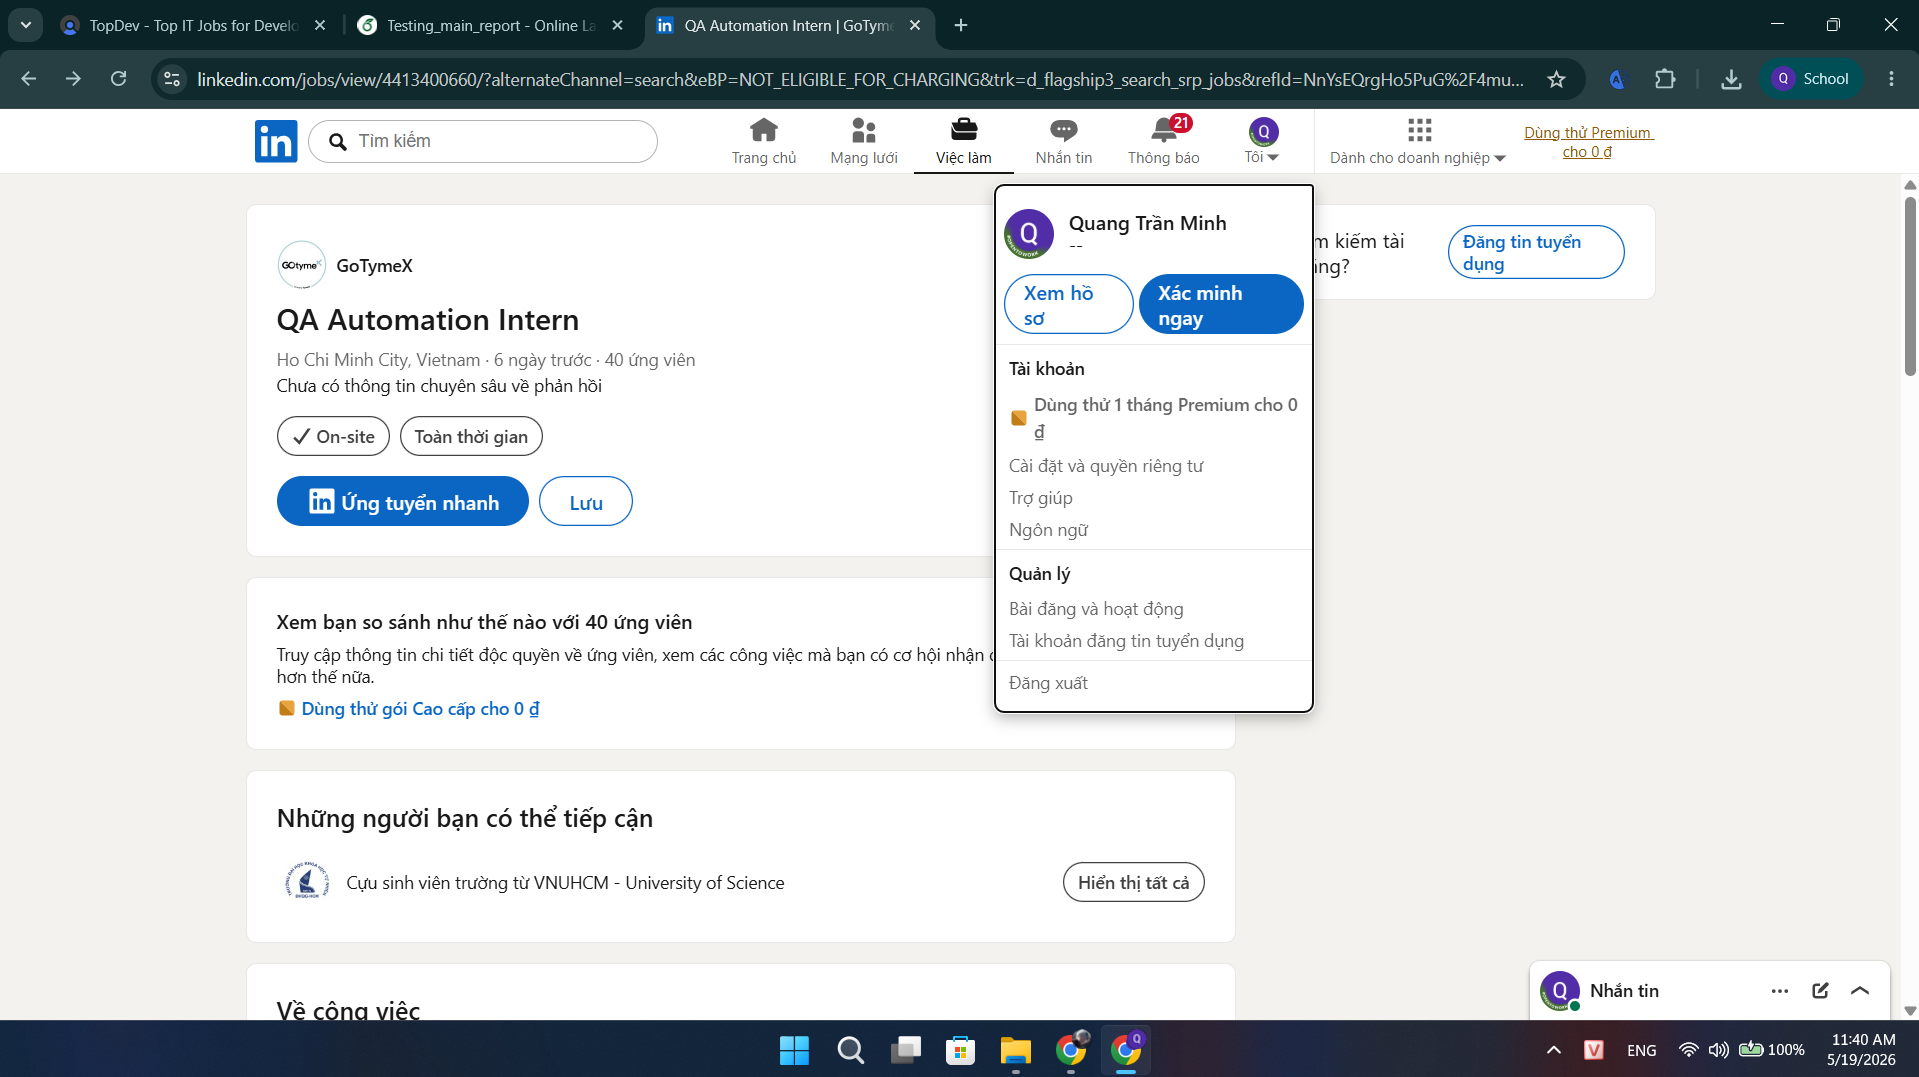
\includegraphics[scale=0.3]{pics_10_QA_QC/QA Automation Intern_GoTymex.png}
\end{center}

\subsubsection{Mô tả công việc}

\begin{center}
    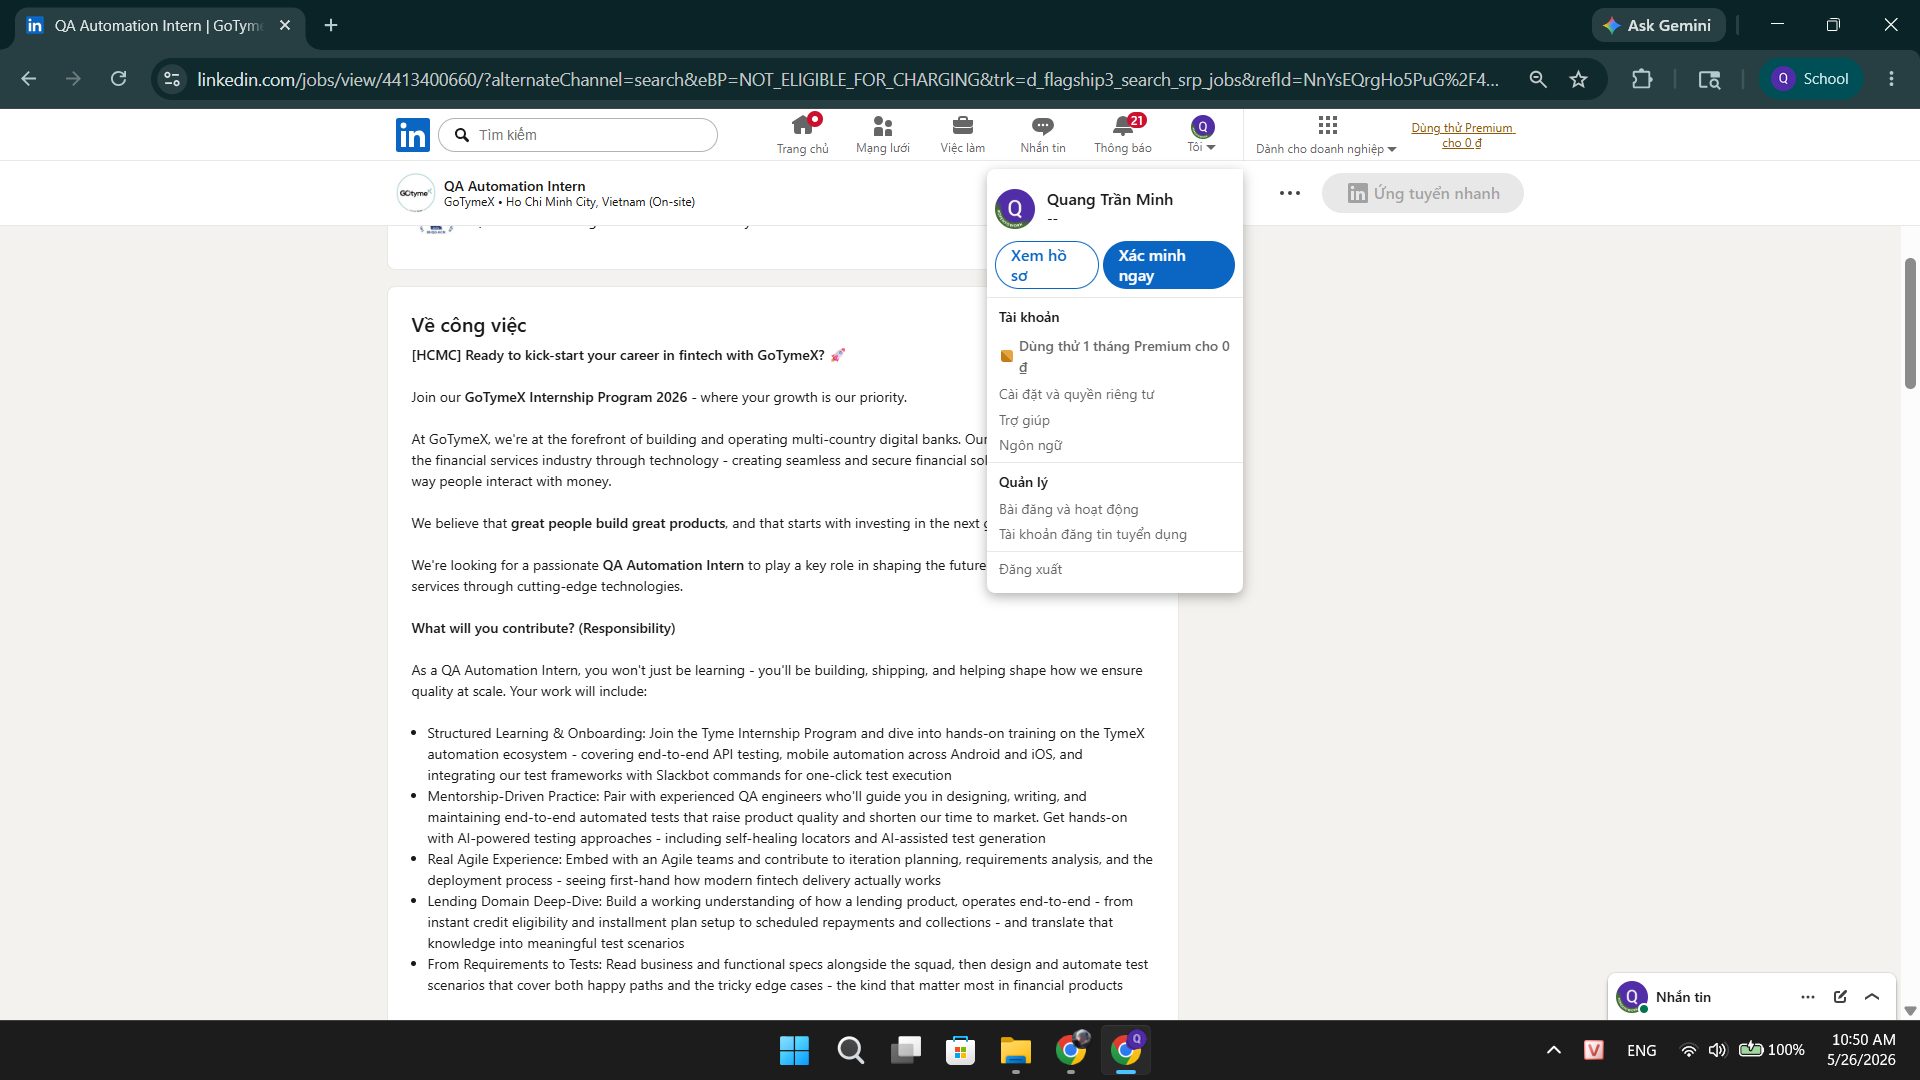
\includegraphics[scale=0.3]{pics_10_QA_QC_des/QA_Automation_Intern_des.png}
\end{center}


\subsubsection{Các kĩ năng yêu cầu}

\begin{center}
    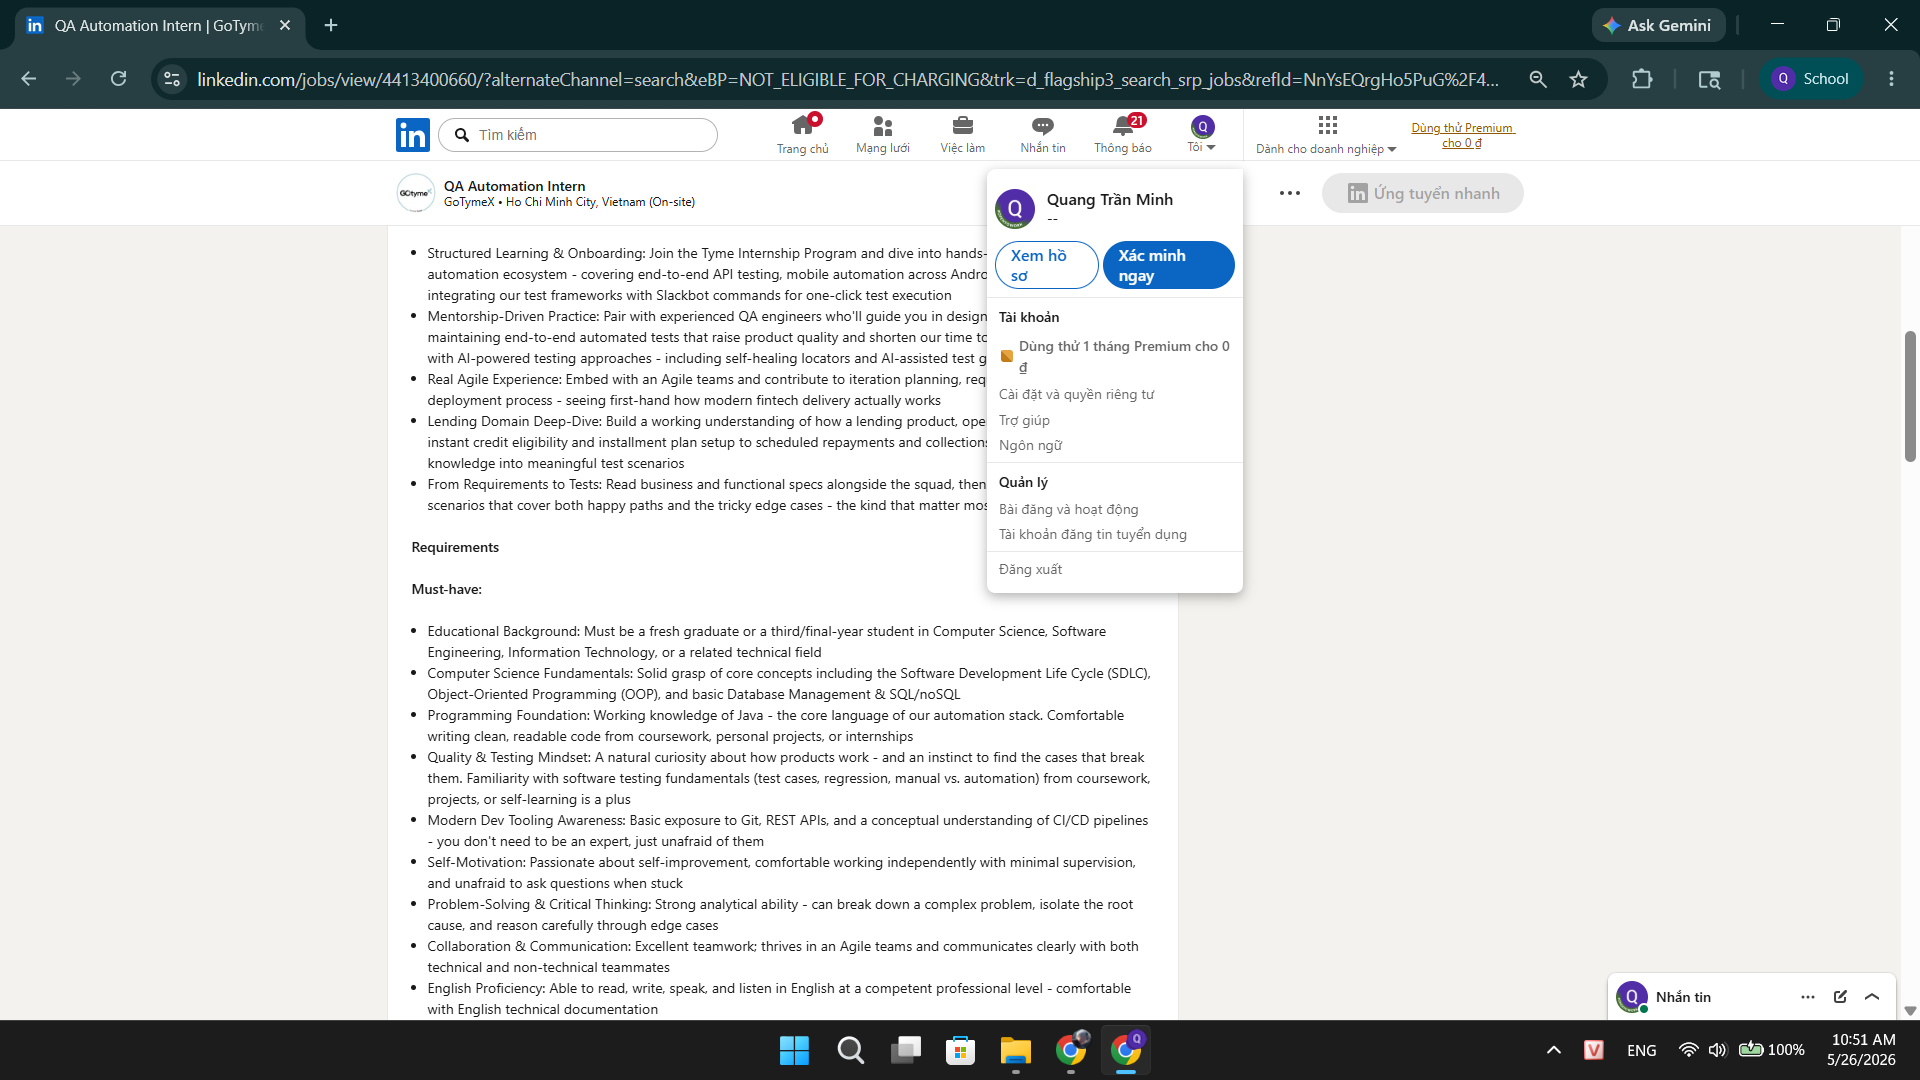
\includegraphics[scale=0.3]{pics_10_QA_QC_skilled/QA_Automation_Intern_skilled_musthave.png}
\end{center}

\vspace{0.5cm} % Thêm một chút khoảng trống giữa 2 phần cho dễ nhìn

\begin{center}
    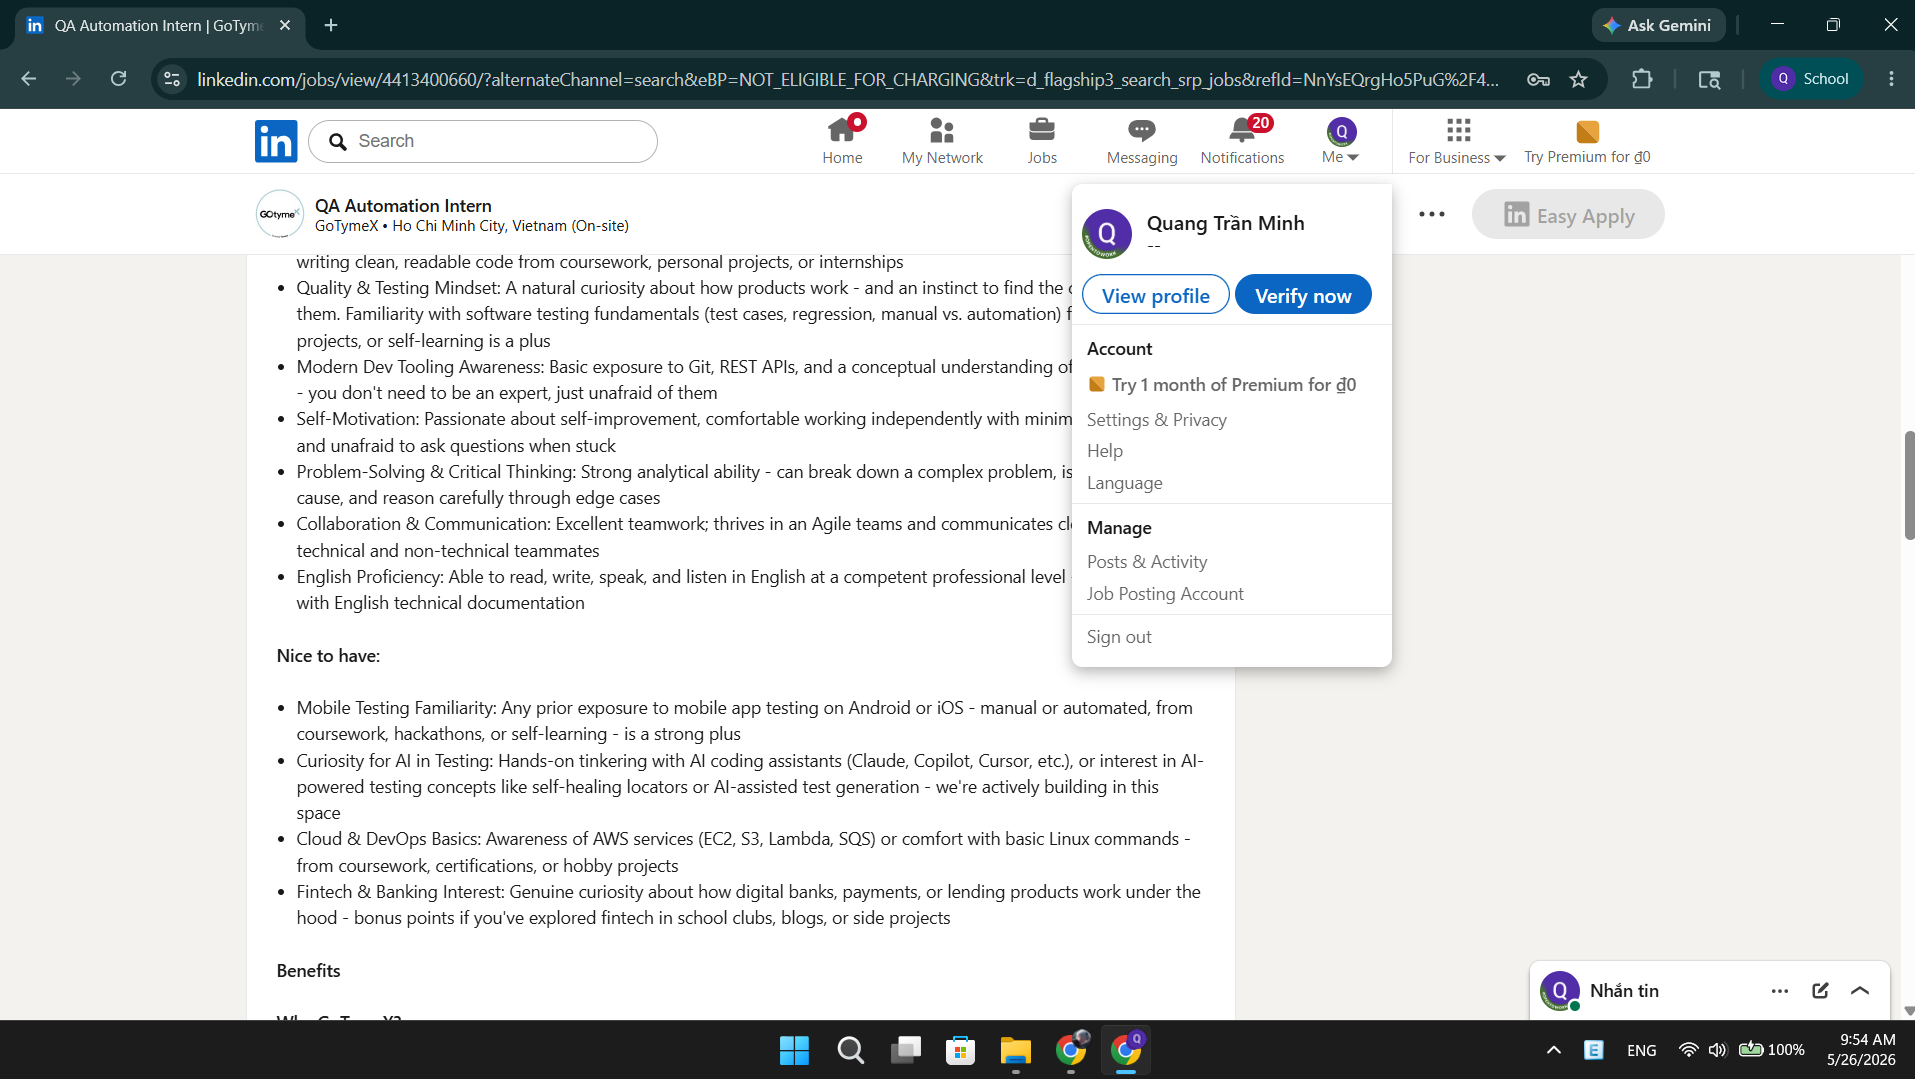
\includegraphics[scale=0.3]{pics_10_QA_QC_skilled/QA_Automation_Intern_skilled_nicehave.png}
\end{center}

\subsubsection{Mức lương}

Allowance: 6,000,000 VND per month (gross)

Meal allowance: 730,000 VND per month

\subsubsection{Phân tích tác động của AI}

Dựa trên mô tả công việc \textbf{"QA Automation Intern"}, ta nhận thấy được rằng trọng tâm của công việc không chỉ có trình bày các kịch bản test một cách thủ công mà thay vào đó là áp dụng các công cụ AI hỗ trợ như: \textbf{self-healing locators, AI-assisted test generation},... những công cụ này sẽ giúp thực tập sinh làm việc một cách hiệu quả. Dưới những tác động của AI như thế đã dẫn đến các thực tập sinh nên có khả năng cộng tác với các mô hình AI như (Claude , Copilot , Cursor,....) đây sẽ là một lợi thế cũng như là thách thức đầu vào của các ứng viên.

\subsection{QC / QA Engineer} 

\subsubsection{Đường dẫn công việc}
\href{https://topdev.vn/detail-jobs/qc-qa-engineer-cong-ty-tnhh-phan-mem-seatos-2102798?src=topdev_home&medium=superhotjobs}{QC / QA Engineer Link}

\subsubsection{Ảnh chụp màn hình công việc}
\begin{center}
    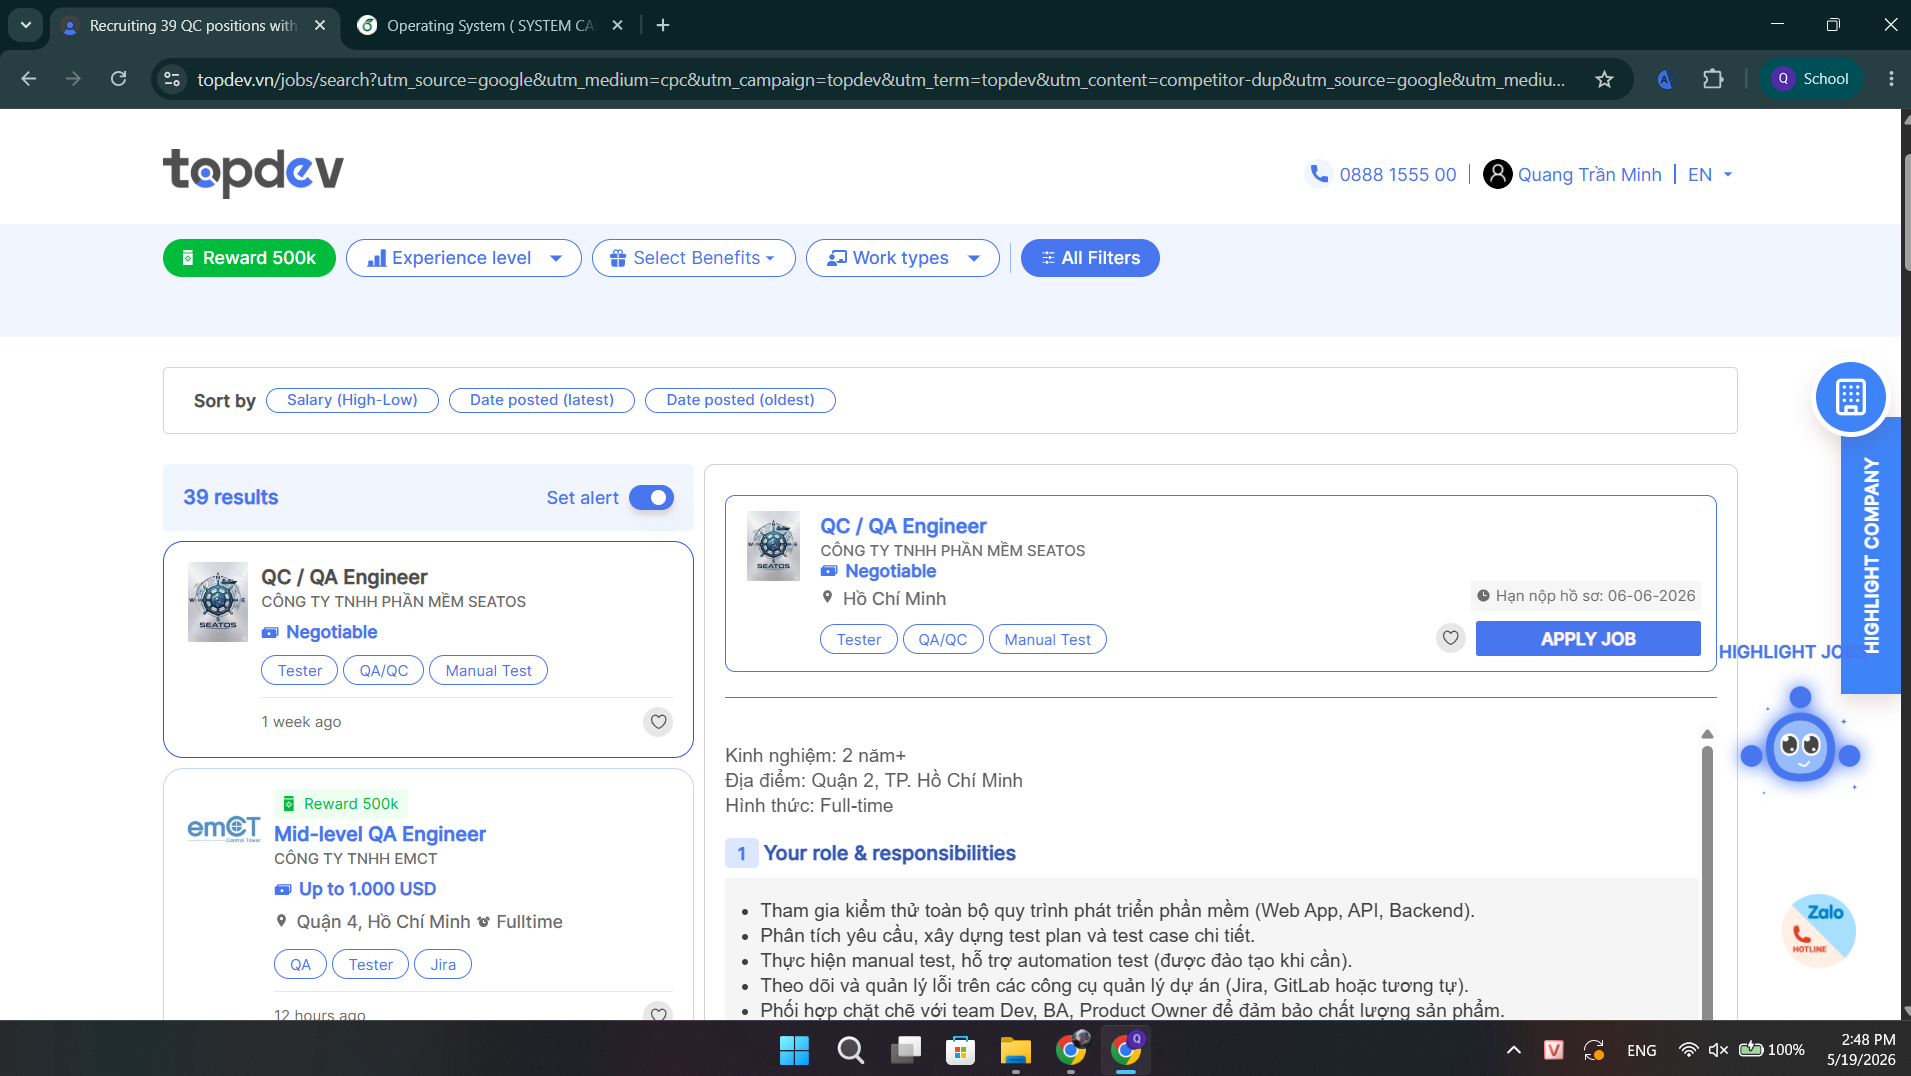
\includegraphics[scale=0.3]{pics_10_QA_QC/QC QA Engineer.png}
\end{center}

\subsubsection{Mô tả công việc}
\begin{center}
    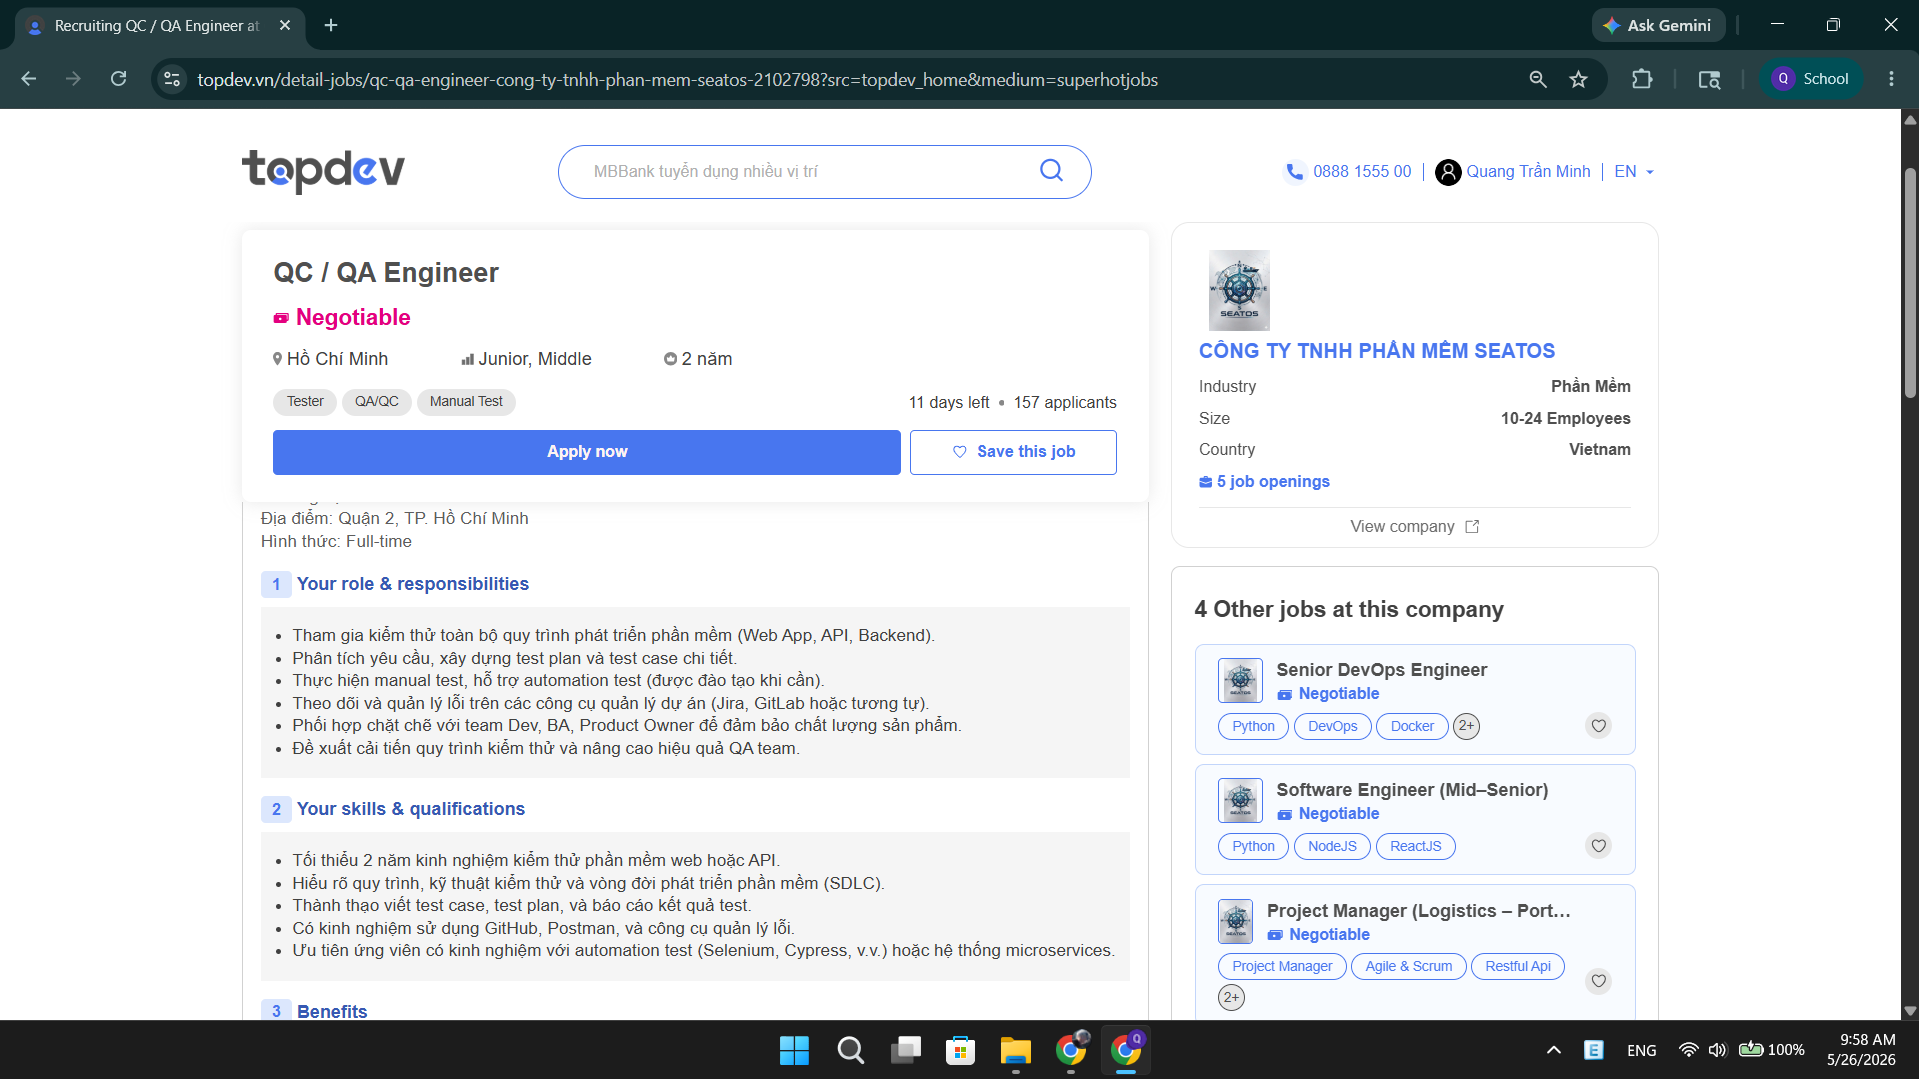
\includegraphics[scale=0.3]{pics_10_QA_QC_des/QC_QA_Engineer_des.png}
\end{center}


\subsubsection{Các kĩ năng yêu cầu}

\begin{center}
    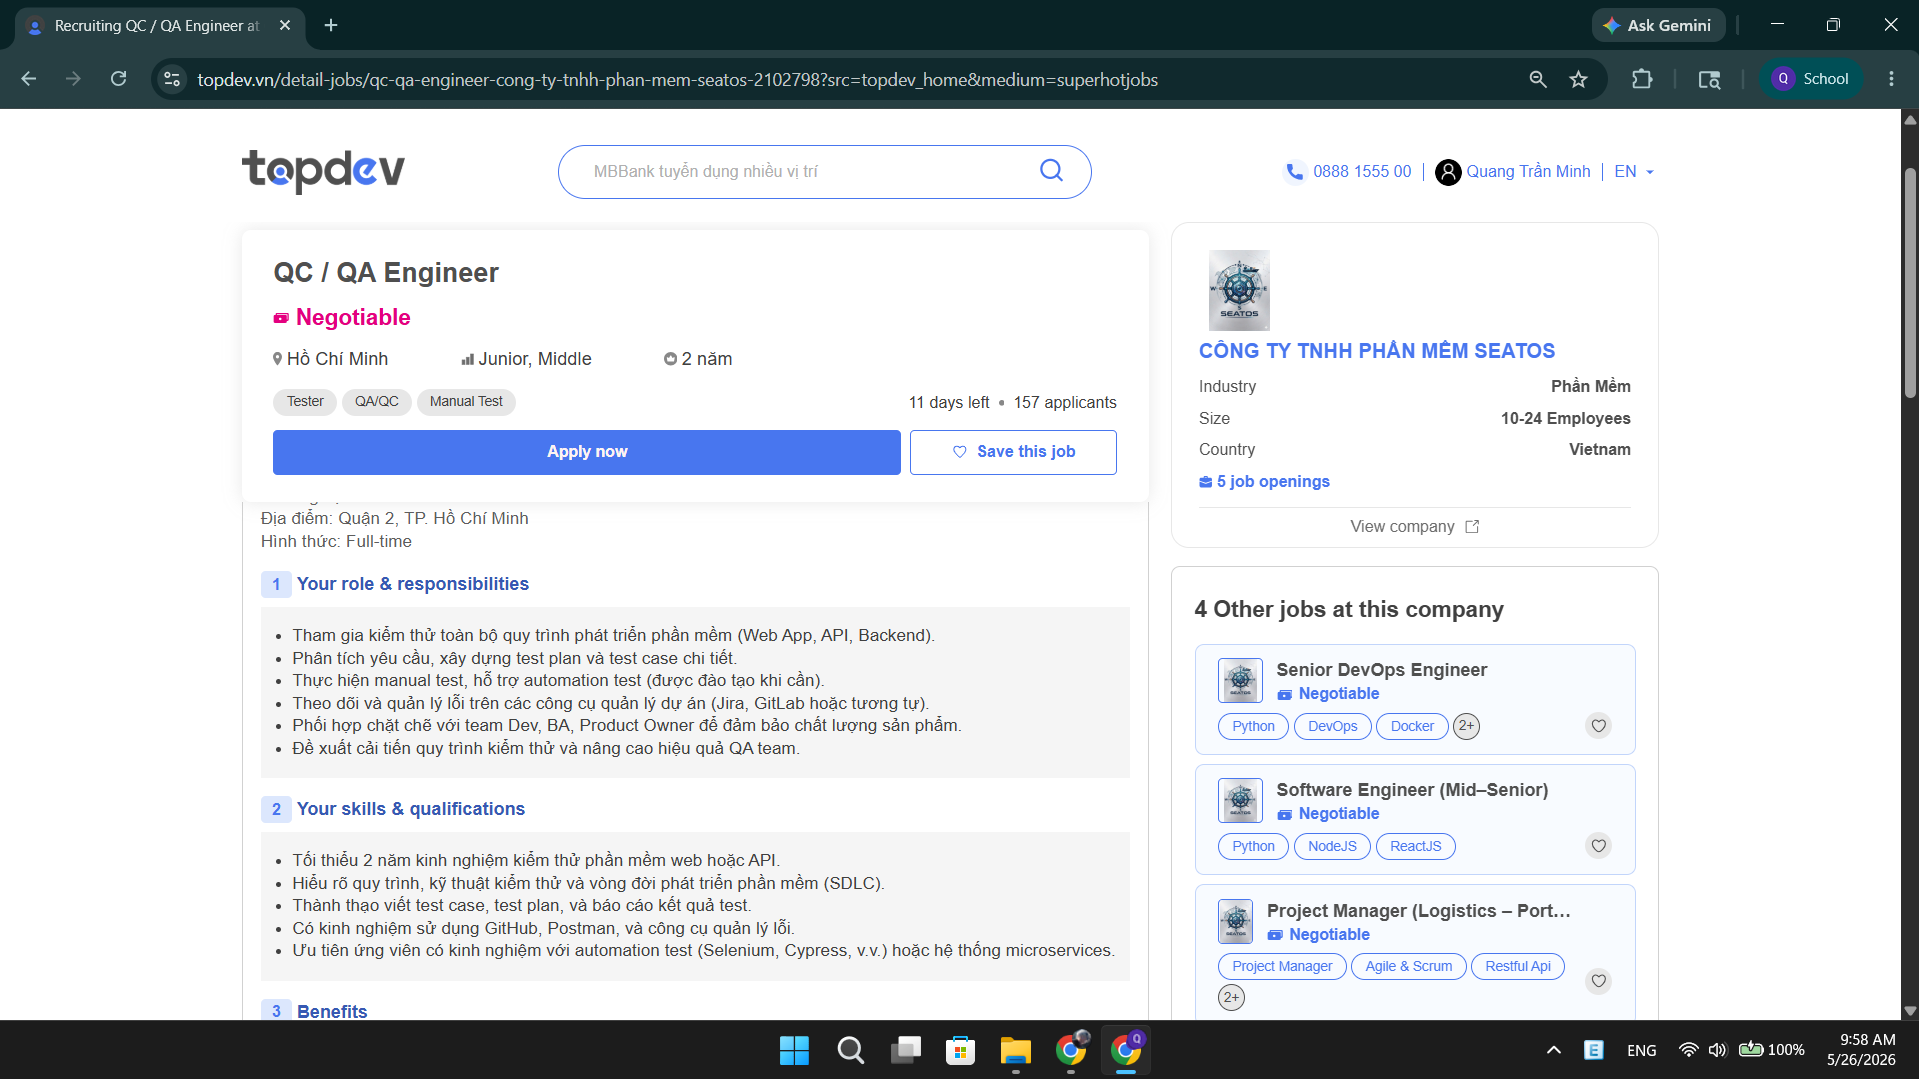
\includegraphics[scale=0.3]{pics_10_QA_QC_skilled/QC_QA_Engineer_skilled.png}
\end{center}

\subsubsection{Mức lương}

Lương cạnh tranh, thỏa thuận theo năng lực. 

\subsubsection{Phân tích tác động của AI}

Đưa ra thông tin về mô tả công việc cùng các kỹ năng cần thiết cho vị trí  \textbf{"QC/QA Engineer"}, nếu là ứng viên đã có kinh nghiệm ít nhất 2 năm trong thời kỳ AI, thì viết \textbf{"manual test"} sẽ trở nên không có giá trị mà thay vào đó họ cần biết cách tận dụng AI để tạo thử nghiệm và phân tích.  Mặt khác, trong mô tả công việc không nói gì về việc sử dụng các công cụ hỗ trợ
từ AI khi làm việc như: \textbf{self-healing locators, AI-assisted test generation},... thì hình ảnh của doanh
nghiệp sẽ không được đánh giá cao và khả năng tạo hứng thú đối với vị trí công việc ở ứng viên
sẽ trở nên hạn chế.

\subsection{Mid-level QA Engineer} 

\subsubsection{Đường dẫn công việc}
\href{https://topdev.vn/detail-jobs/mid-level-qa-engineer-cong-ty-tnhh-emct-2102215?src=topdev_home&medium=superhotjobs}{Mid-level QA Engineer Link}

\subsubsection{Ảnh chụp màn hình công việc}
\begin{center}
    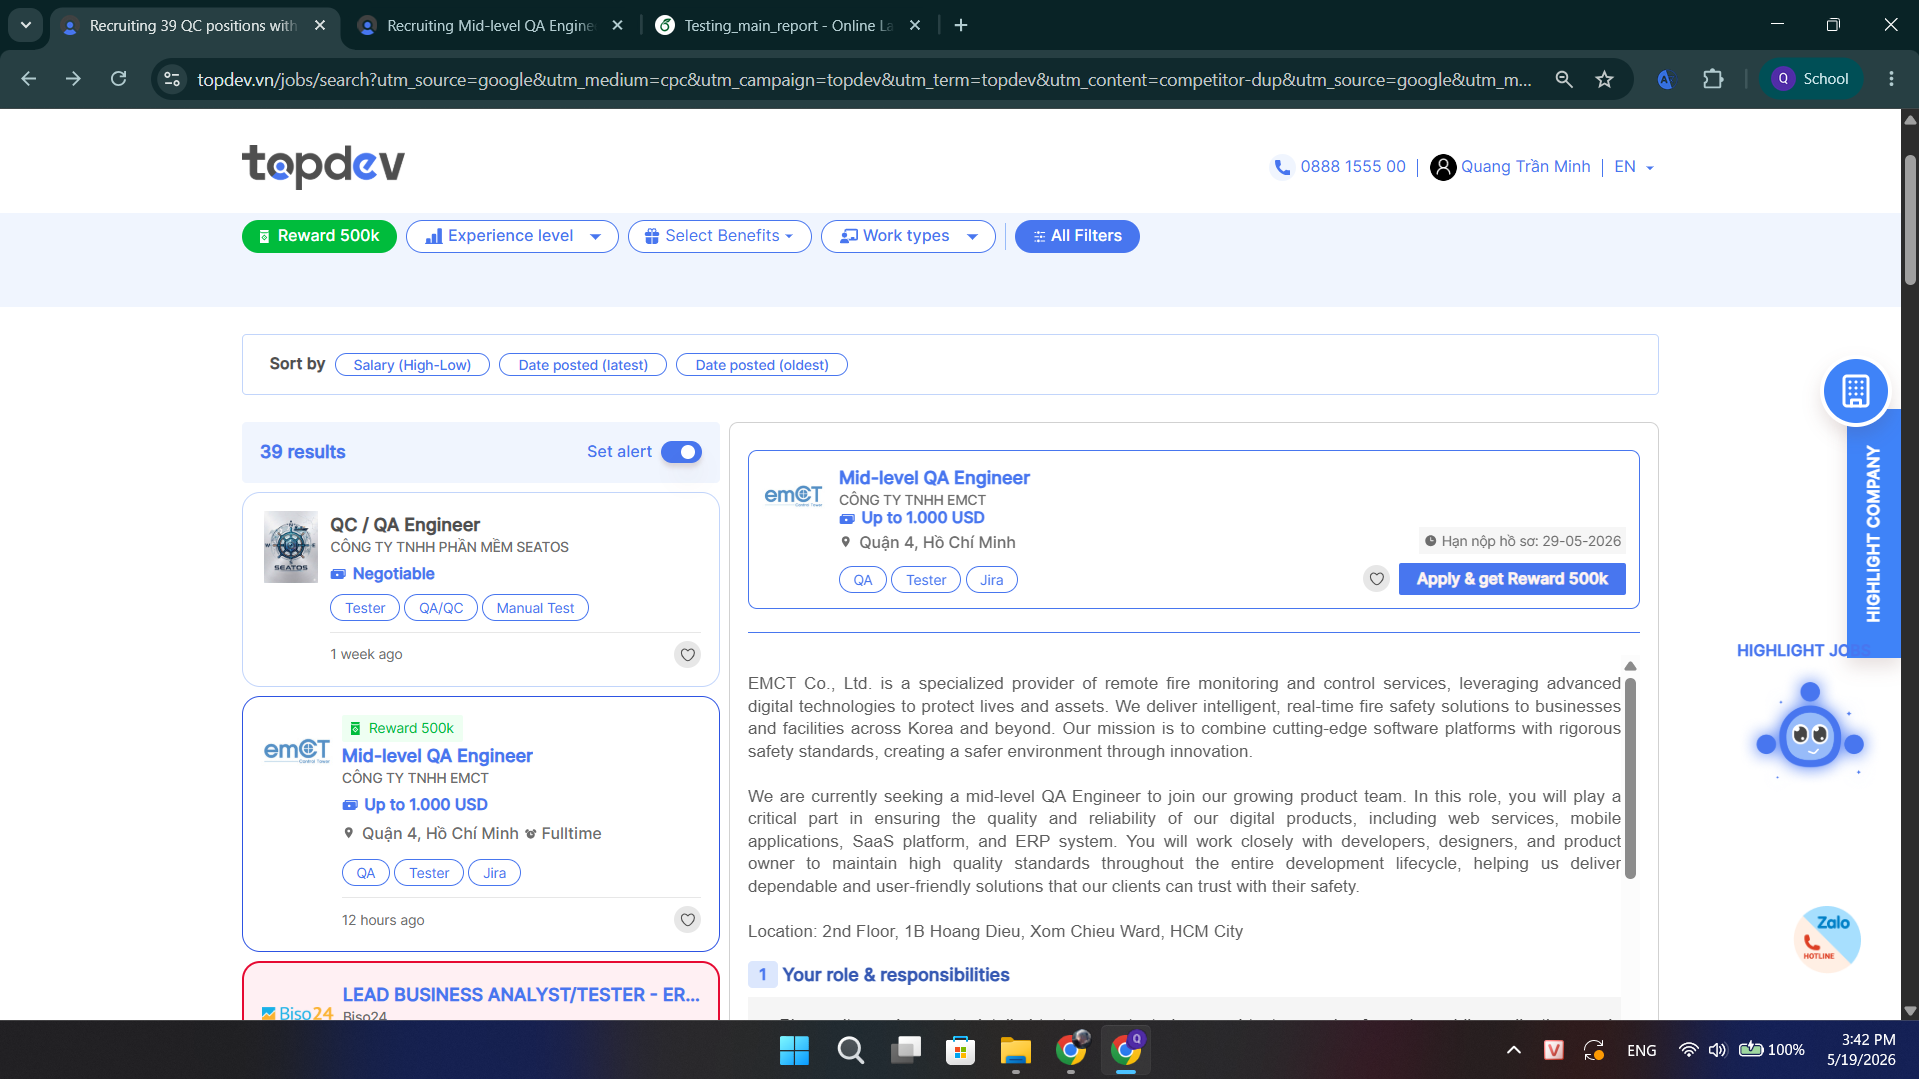
\includegraphics[scale=0.3]{pics_10_QA_QC/Mid-level QA Engineer.png}
\end{center}

\subsubsection{Mô tả công việc}
\begin{center}
    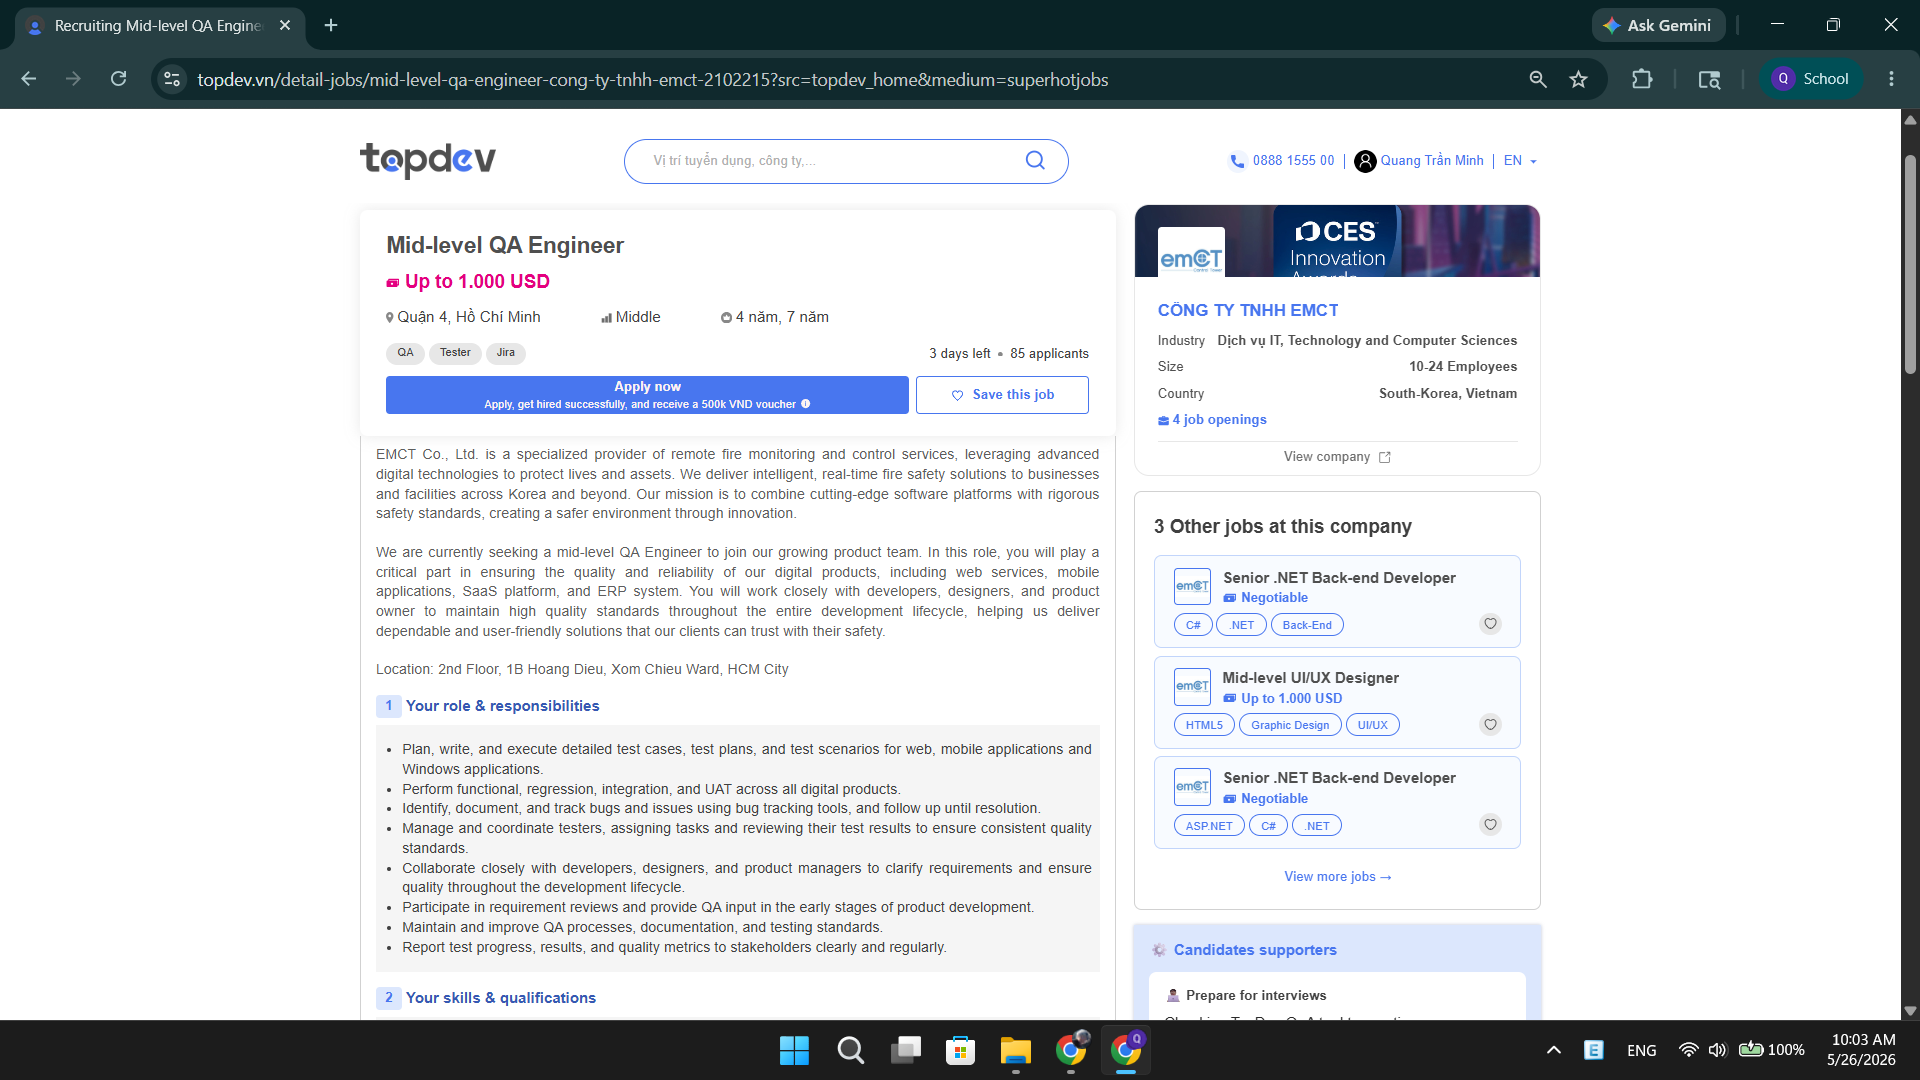
\includegraphics[scale=0.3]{pics_10_QA_QC_des/Mid-level_QA_Engineer_des.png}
\end{center}

\subsubsection{Các kĩ năng yêu cầu}

\begin{center}
    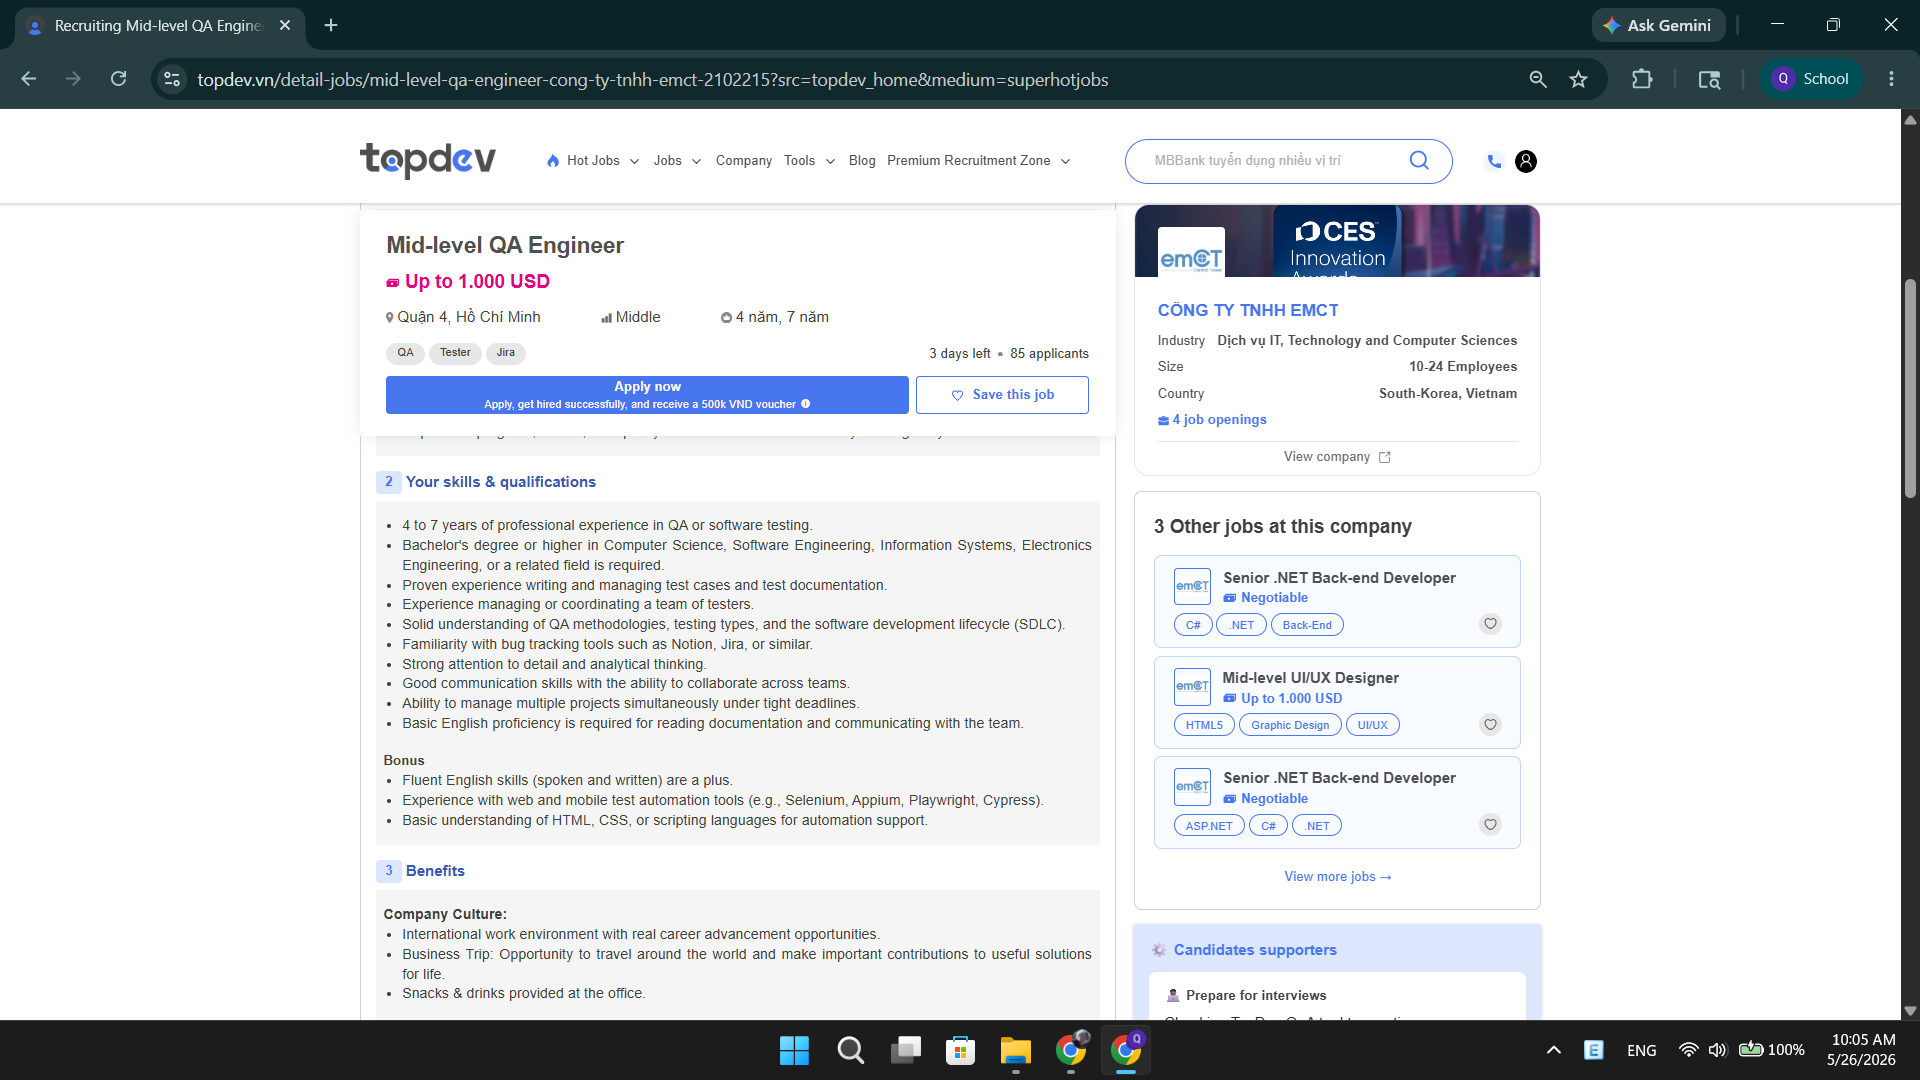
\includegraphics[scale=0.3]{pics_10_QA_QC_skilled/Mid-level_QA_Engineer_skilled.png}
\end{center}

\subsubsection{Mức lương}

Salary range in Gross: up to 1,000 USD

Social Insurance and 13th month bonus 

\subsubsection{Phân tích tác động của AI}

AI tác động mạnh đến vị trí Mid-level QA Engineer này bằng cách tự động hóa phần lớn công việc liên quan đến test thủ công , khiến các kỹ năng truyền thống như \textbf{"write detailed test cases"} và \textbf{"execute test"} giảm giá trị, thay vào đó đòi hỏi QA phải biết sử dụng AI để phân tích kết quả tự động và quản lý quy trình kiểm thử thông minh hơn. Tuy nhiên, bản mô tả hiện tại hoàn toàn chưa đề cập đến \textbf{AI-powered testing} hay \textbf{automation tools} hiện đại, điều này cho thấy công ty có nguy cơ tụt hậu so với các tổ chức đã tích hợp \textbf{self-healing locators} hay \textbf{AI-assisted test generation} vào quy trình QA.

\subsection{Senior Automation Test Engineer (Playwright, Java, AI)} 

\subsubsection{Đường dẫn công việc}
\href{https://itviec.com/viec-lam-it/senior-automation-test-engineer-playwright-java-ai-hansen-technologies-2646?lab_feature=similar_job}{Senior Automation Test Engineer (Playwright, Java, AI) Link}

\subsubsection{Ảnh chụp màn hình công việc}
\begin{center}
    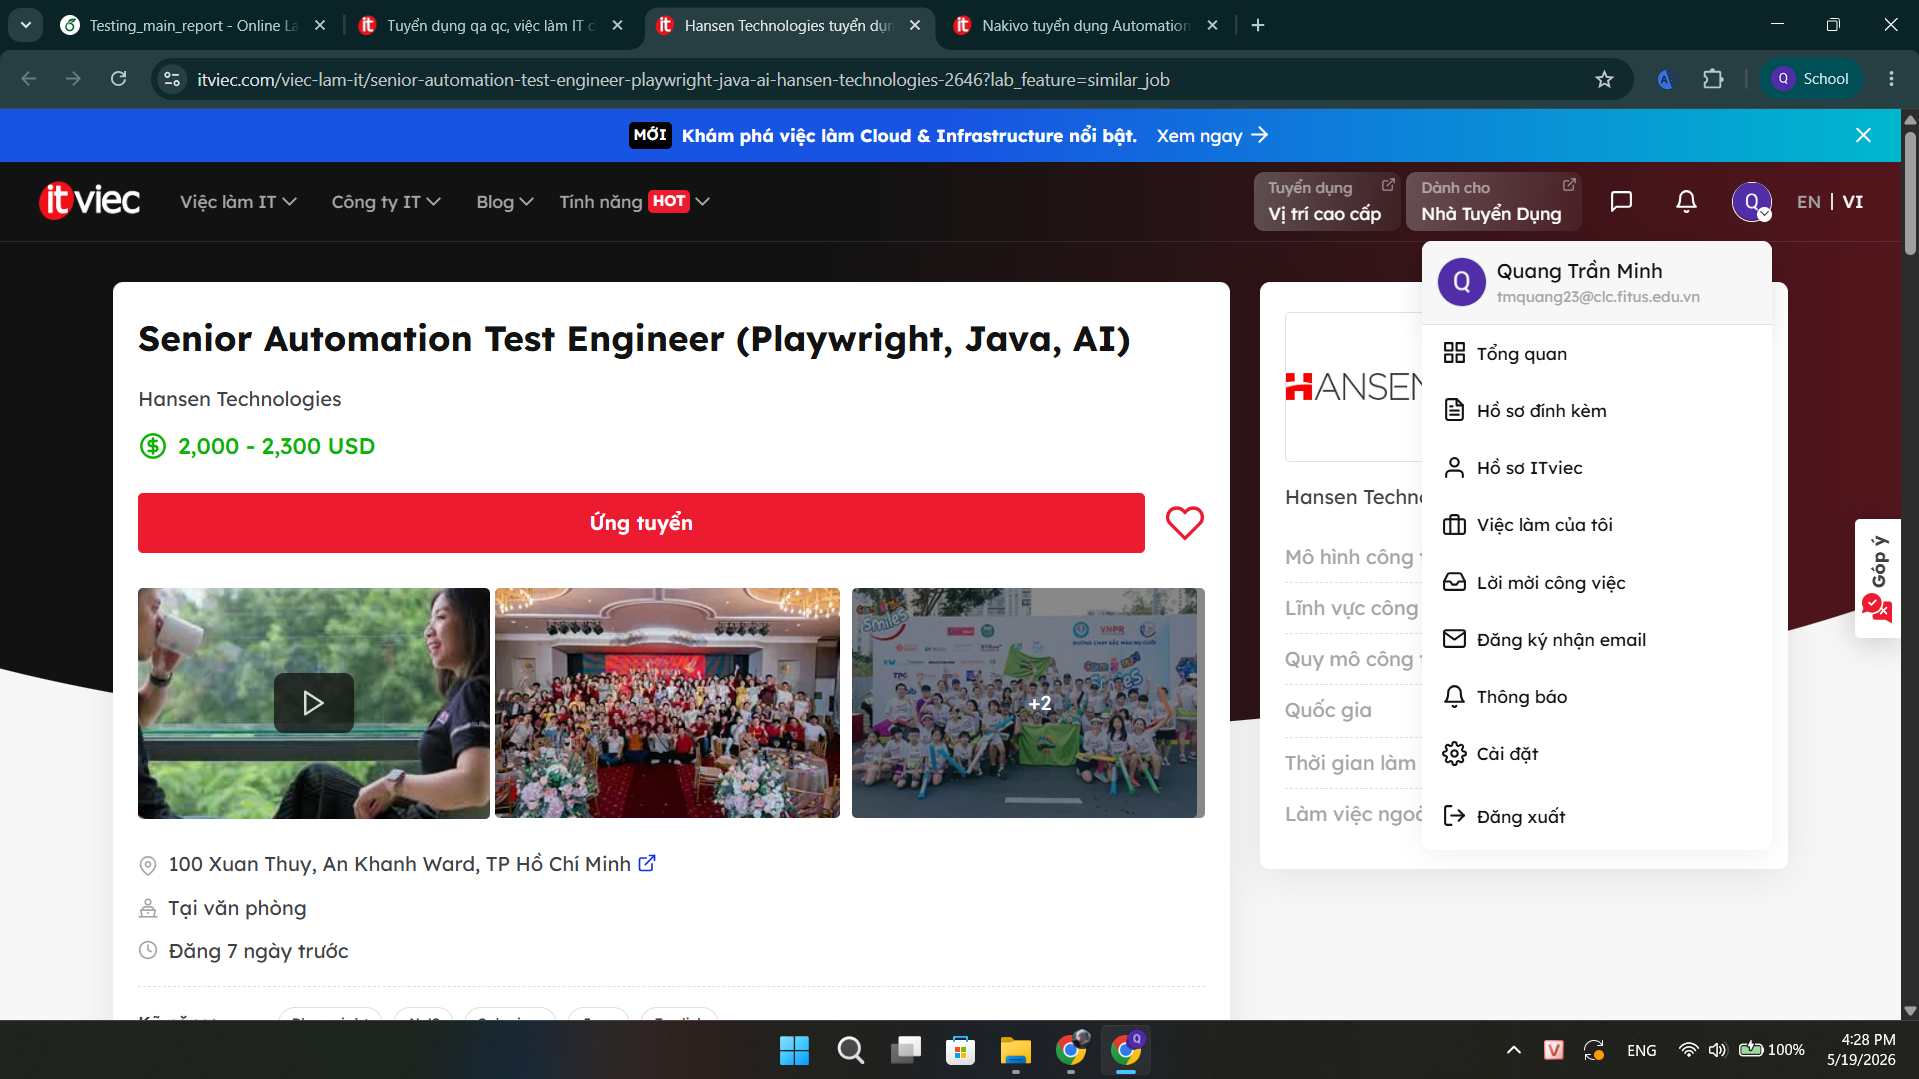
\includegraphics[scale=0.3]{pics_10_QA_QC/Senior Automation Test Engineer (Playwright, Java, AI).png}
\end{center}

\subsubsection{Mô tả công việc}
\begin{center}
    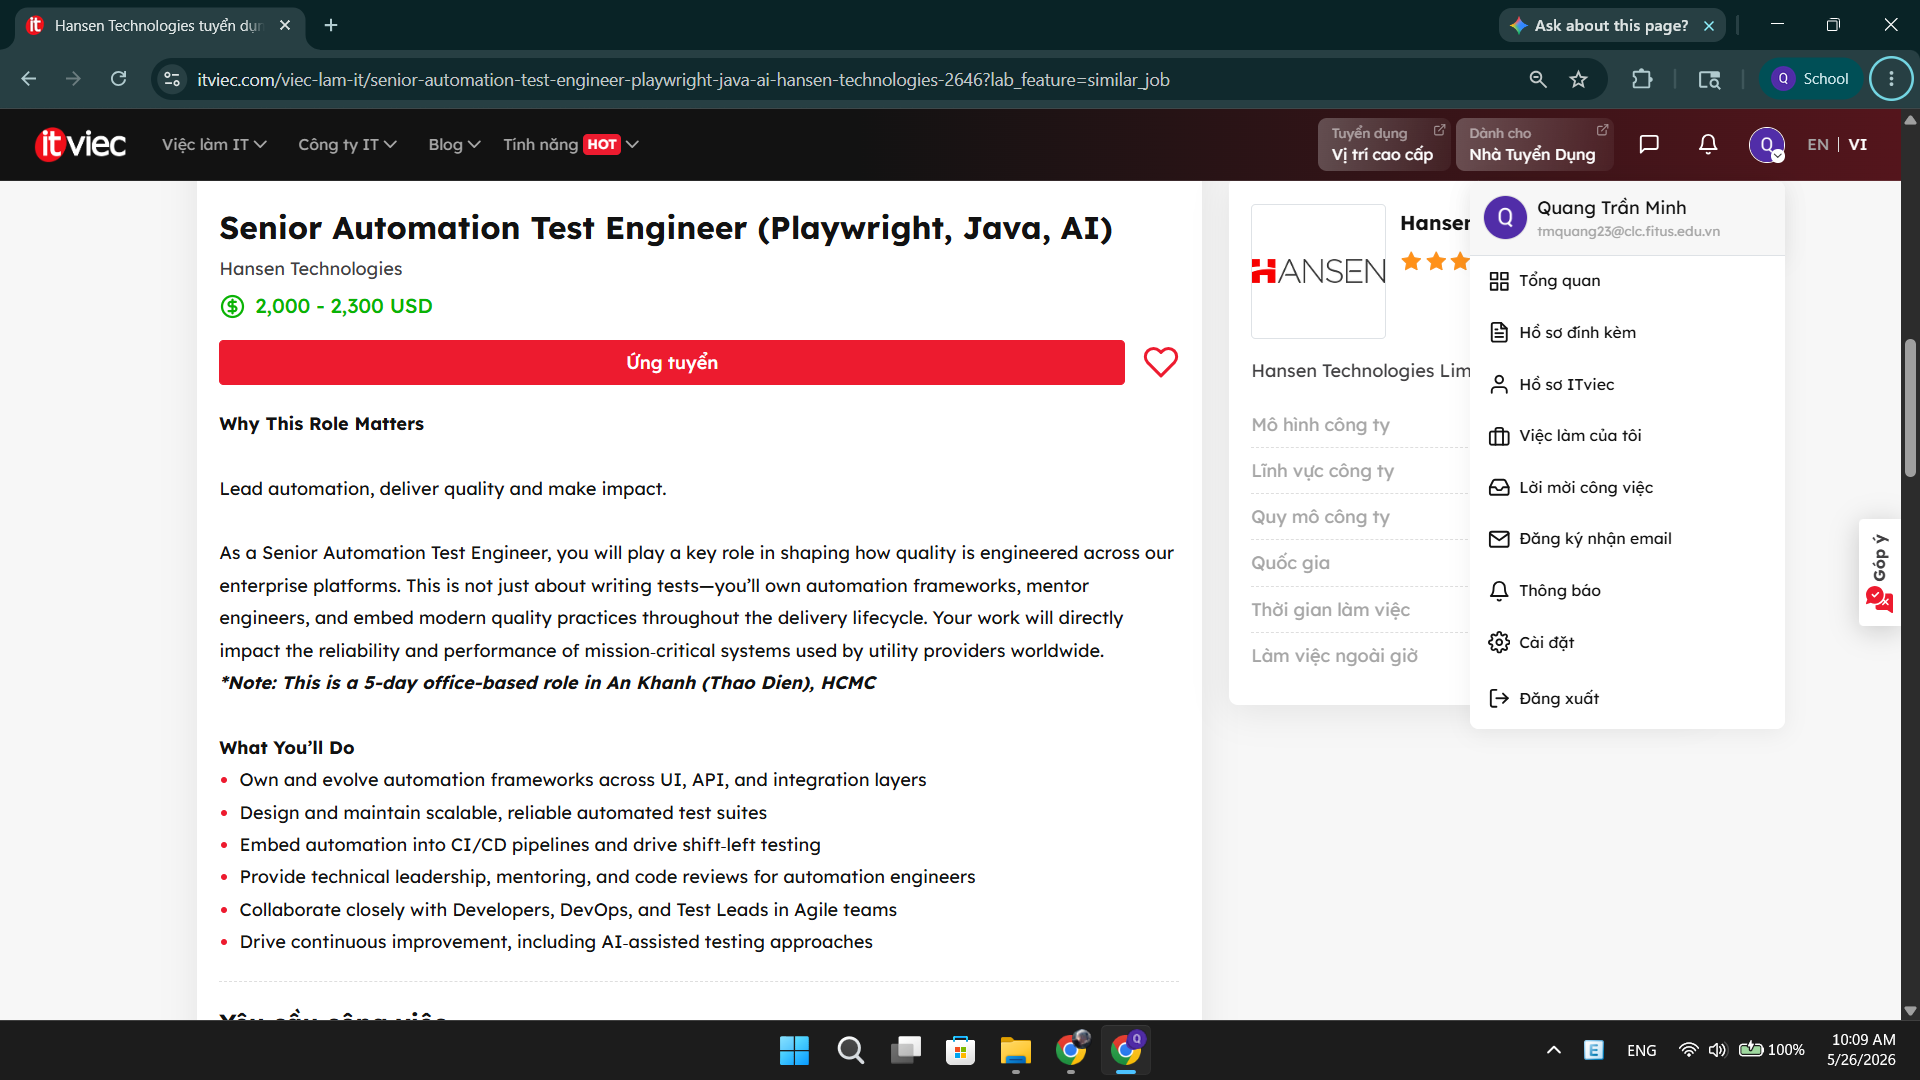
\includegraphics[scale=0.3]{pics_10_QA_QC_des/Senior_Automation_Test_Engineer_des.png}
\end{center}

\subsubsection{Các kĩ năng yêu cầu}
\begin{center}
    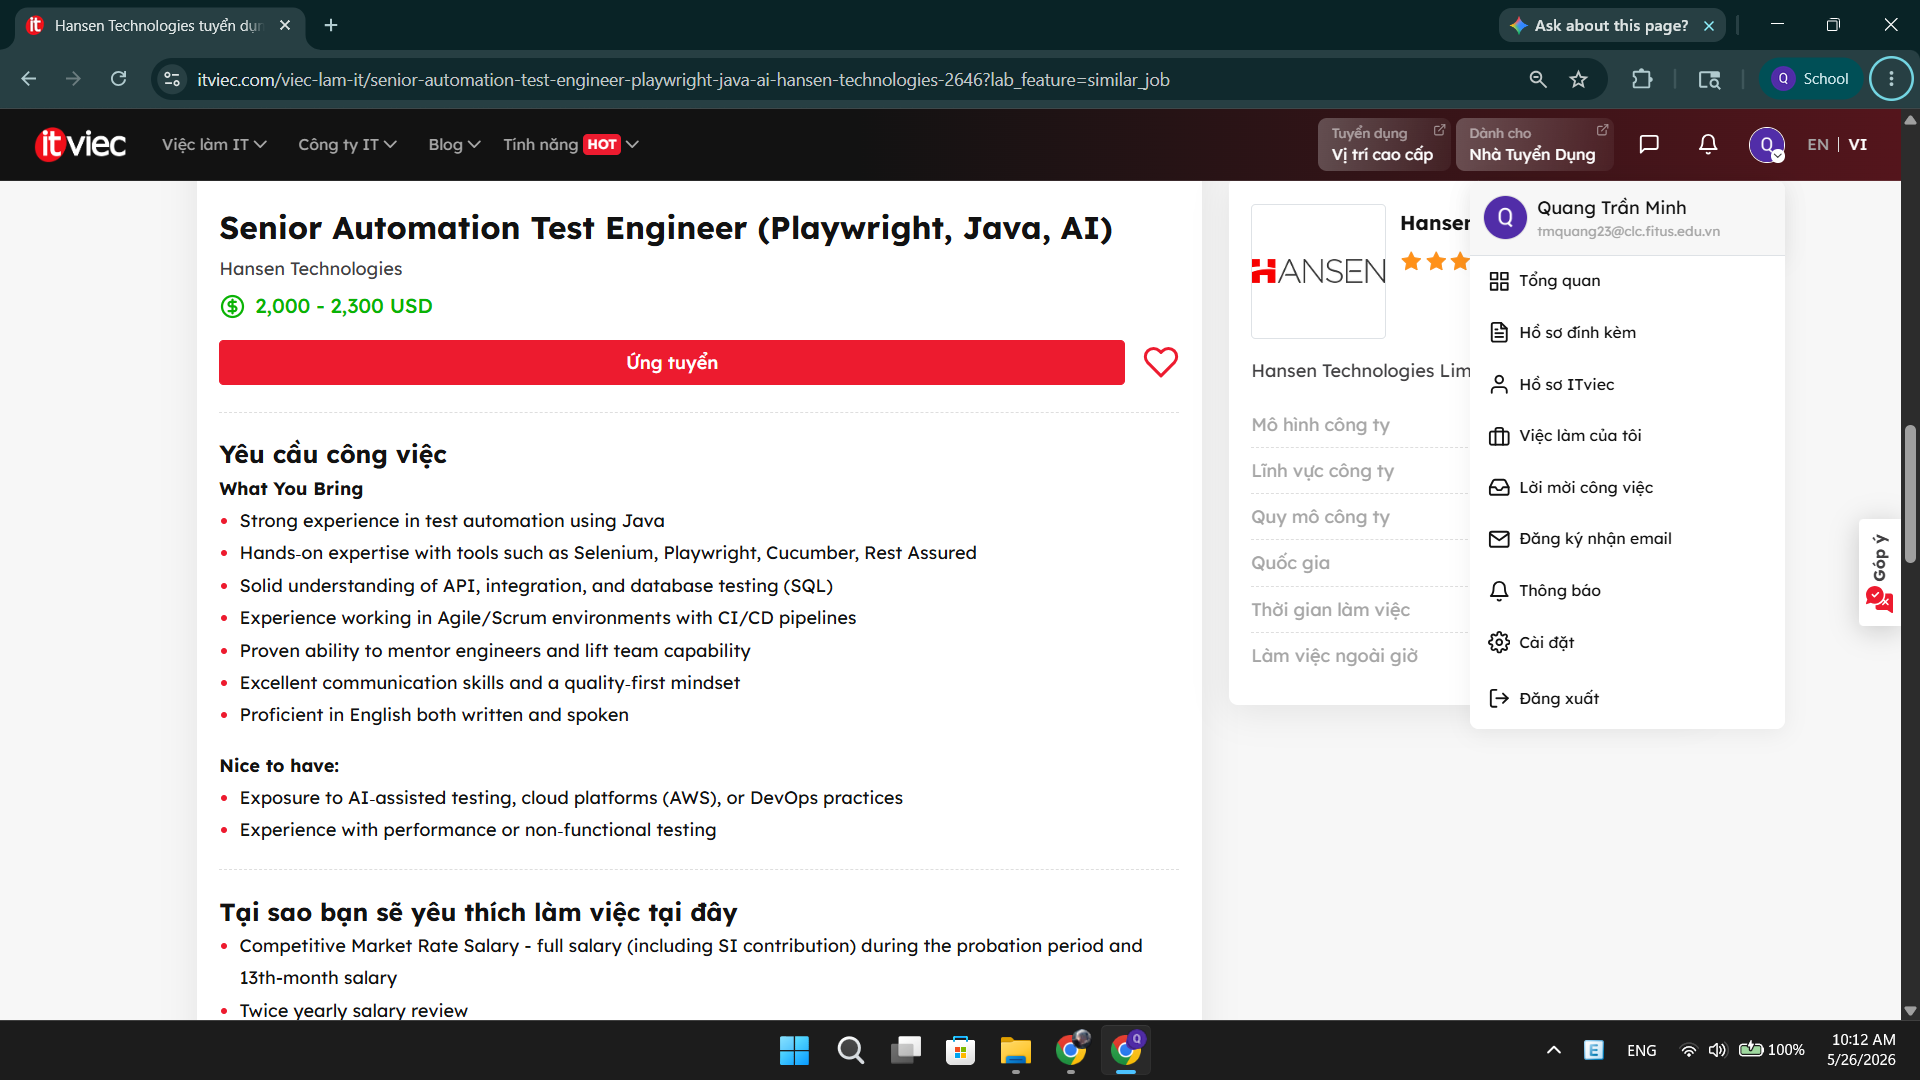
\includegraphics[scale=0.3]{pics_10_QA_QC_skilled/Senior_Automation_Test_Engineer_skilled.png}
\end{center}

\subsubsection{Mức lương}

Salary in range: 2,000 - 2,300 USD 

\subsubsection{Phân tích tác động của AI}

Dựa trên mô tả công việc cũng như yêu cầu kĩ năng, AI tác động mạnh mẽ trong việc yêu cầu các ứng viên Senior cần biết sử dụng AI trong việc tự động sinh test, tối ưu bảo trì framework và phát hiện lỗi thông minh hơn, đồng thời yêu cầu kỹ sư phải cập nhật liên tục các công cụ AI mới. Ngoài ra Senior còn phải biết tích hợp AI vào CI/CD và khai thác AI để kiểm thử nhanh hơn, chính xác hơn.

\subsection{Automation QA Engineer (QA QC/Tester/Automation Test)} 

\subsubsection{Đường dẫn công việc}
\href{https://itviec.com/viec-lam-it/automation-qa-engineer-qa-qc-tester-automation-test-nakivo-0115?lab_feature=preview_jd_page}{Automation QA Engineer (QA QC/Tester/Automation Test) Link}

\subsubsection{Ảnh chụp màn hình công việc}
\begin{center}
    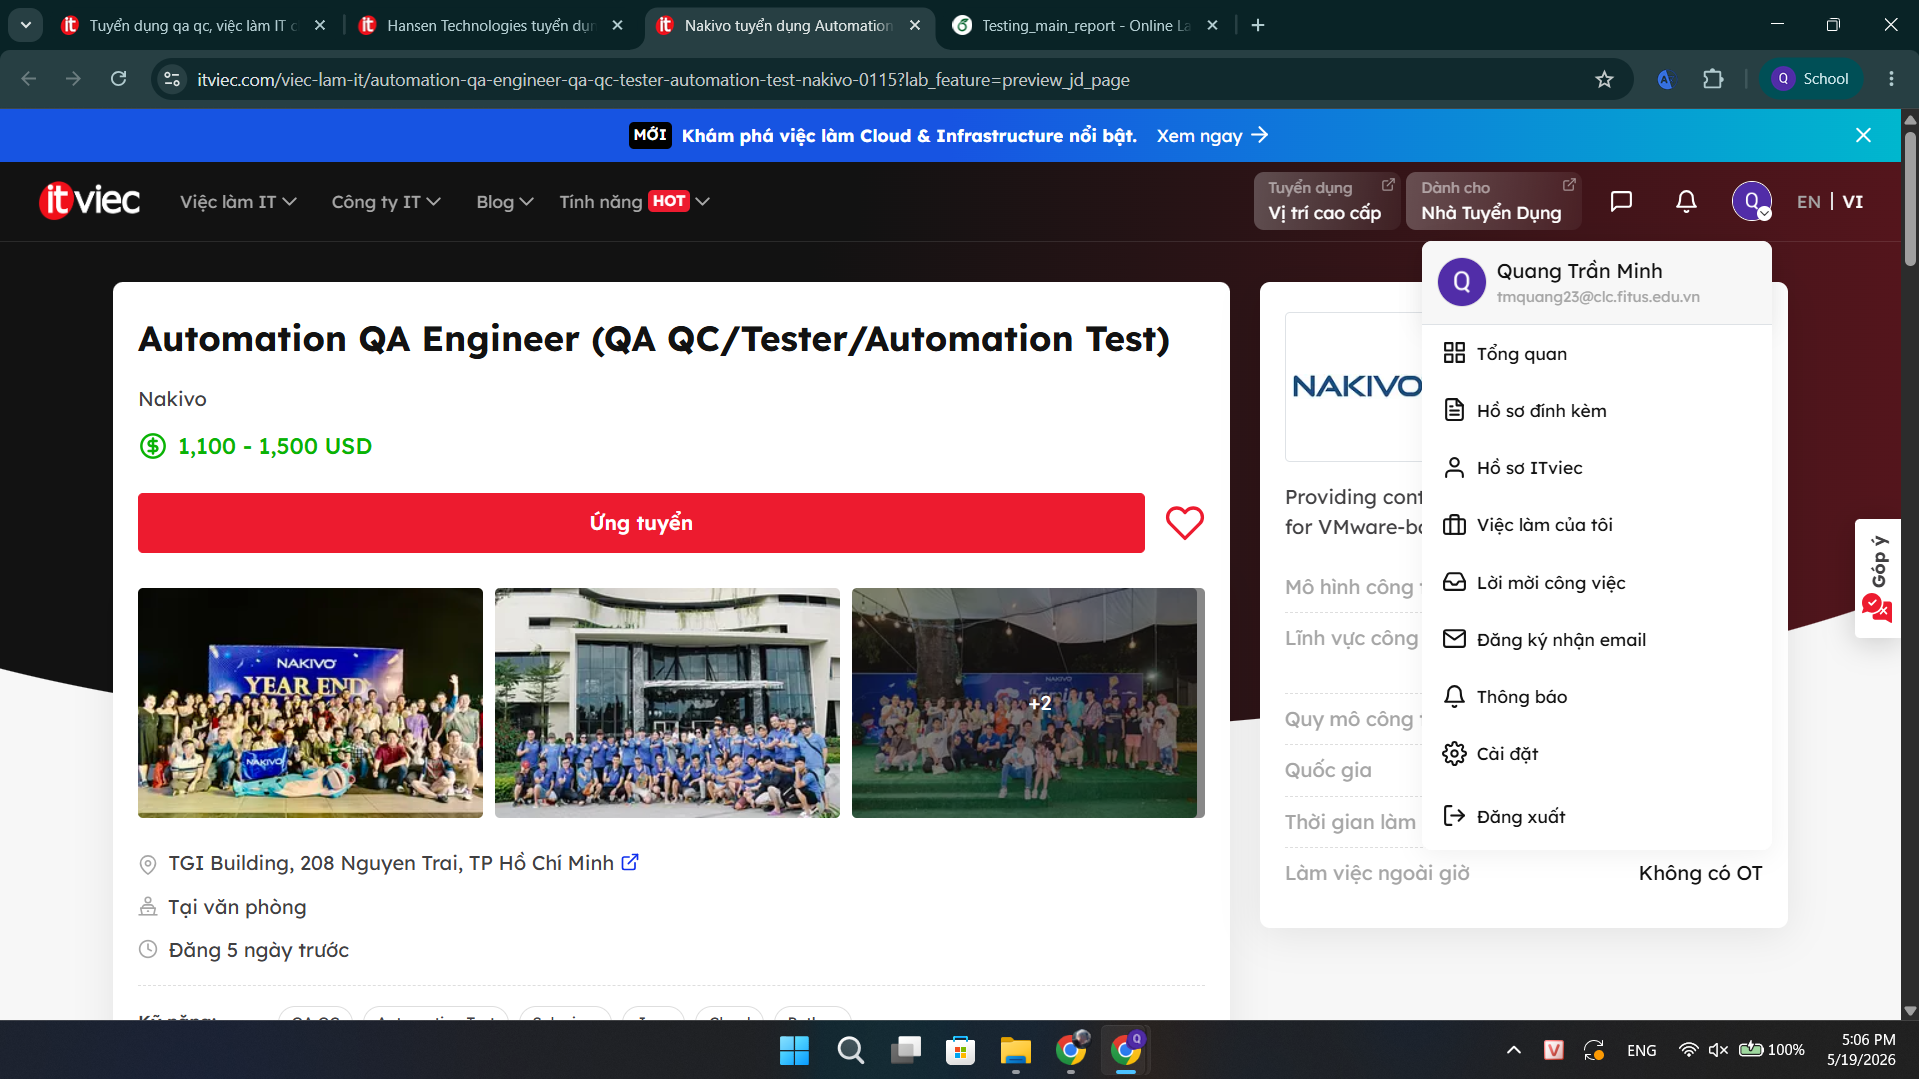
\includegraphics[scale=0.3]{pics_10_QA_QC/Automation QA Engineer (QA QC Tester Automation Test).png}
\end{center}

\subsubsection{Mô tả công việc}
\begin{center}
    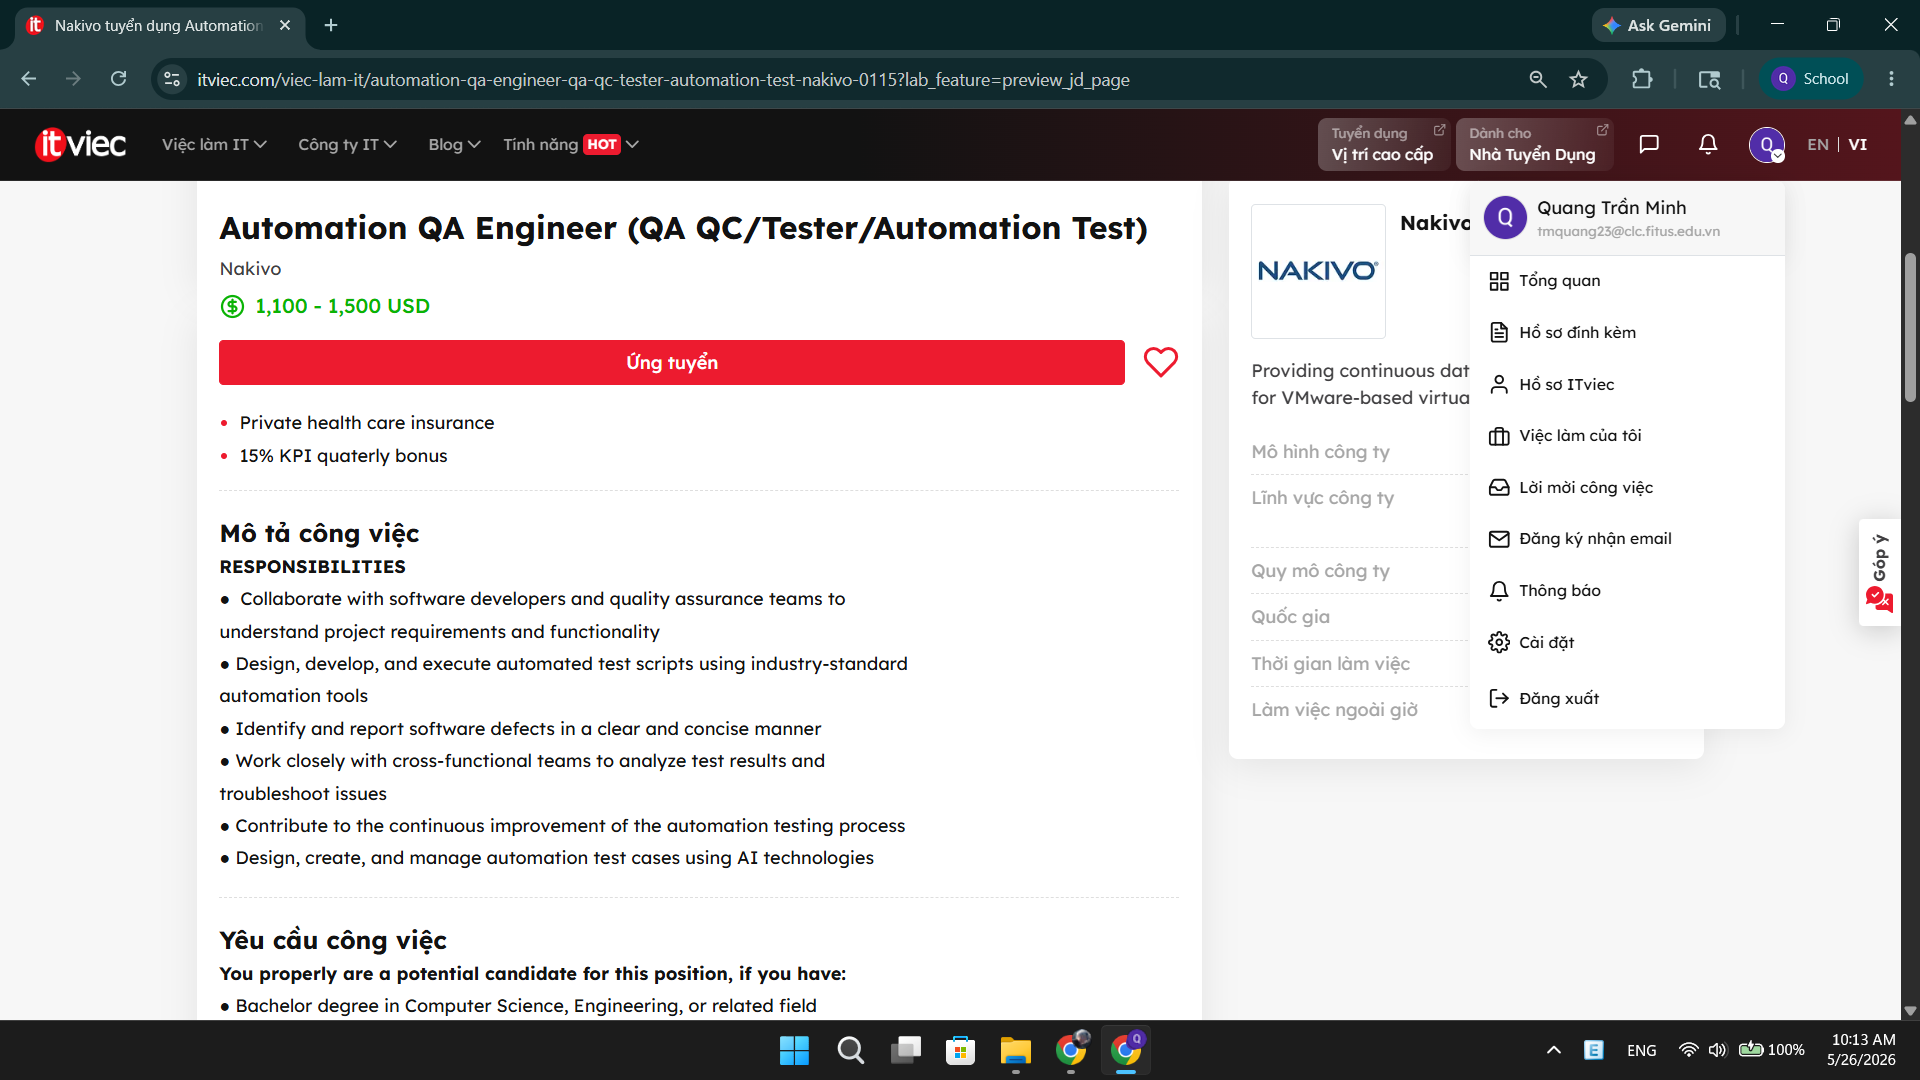
\includegraphics[scale=0.3]{pics_10_QA_QC_des/Automation_QA_Engineer_des.png}
\end{center}

\subsubsection{Các kĩ năng yêu cầu}

\begin{center}
    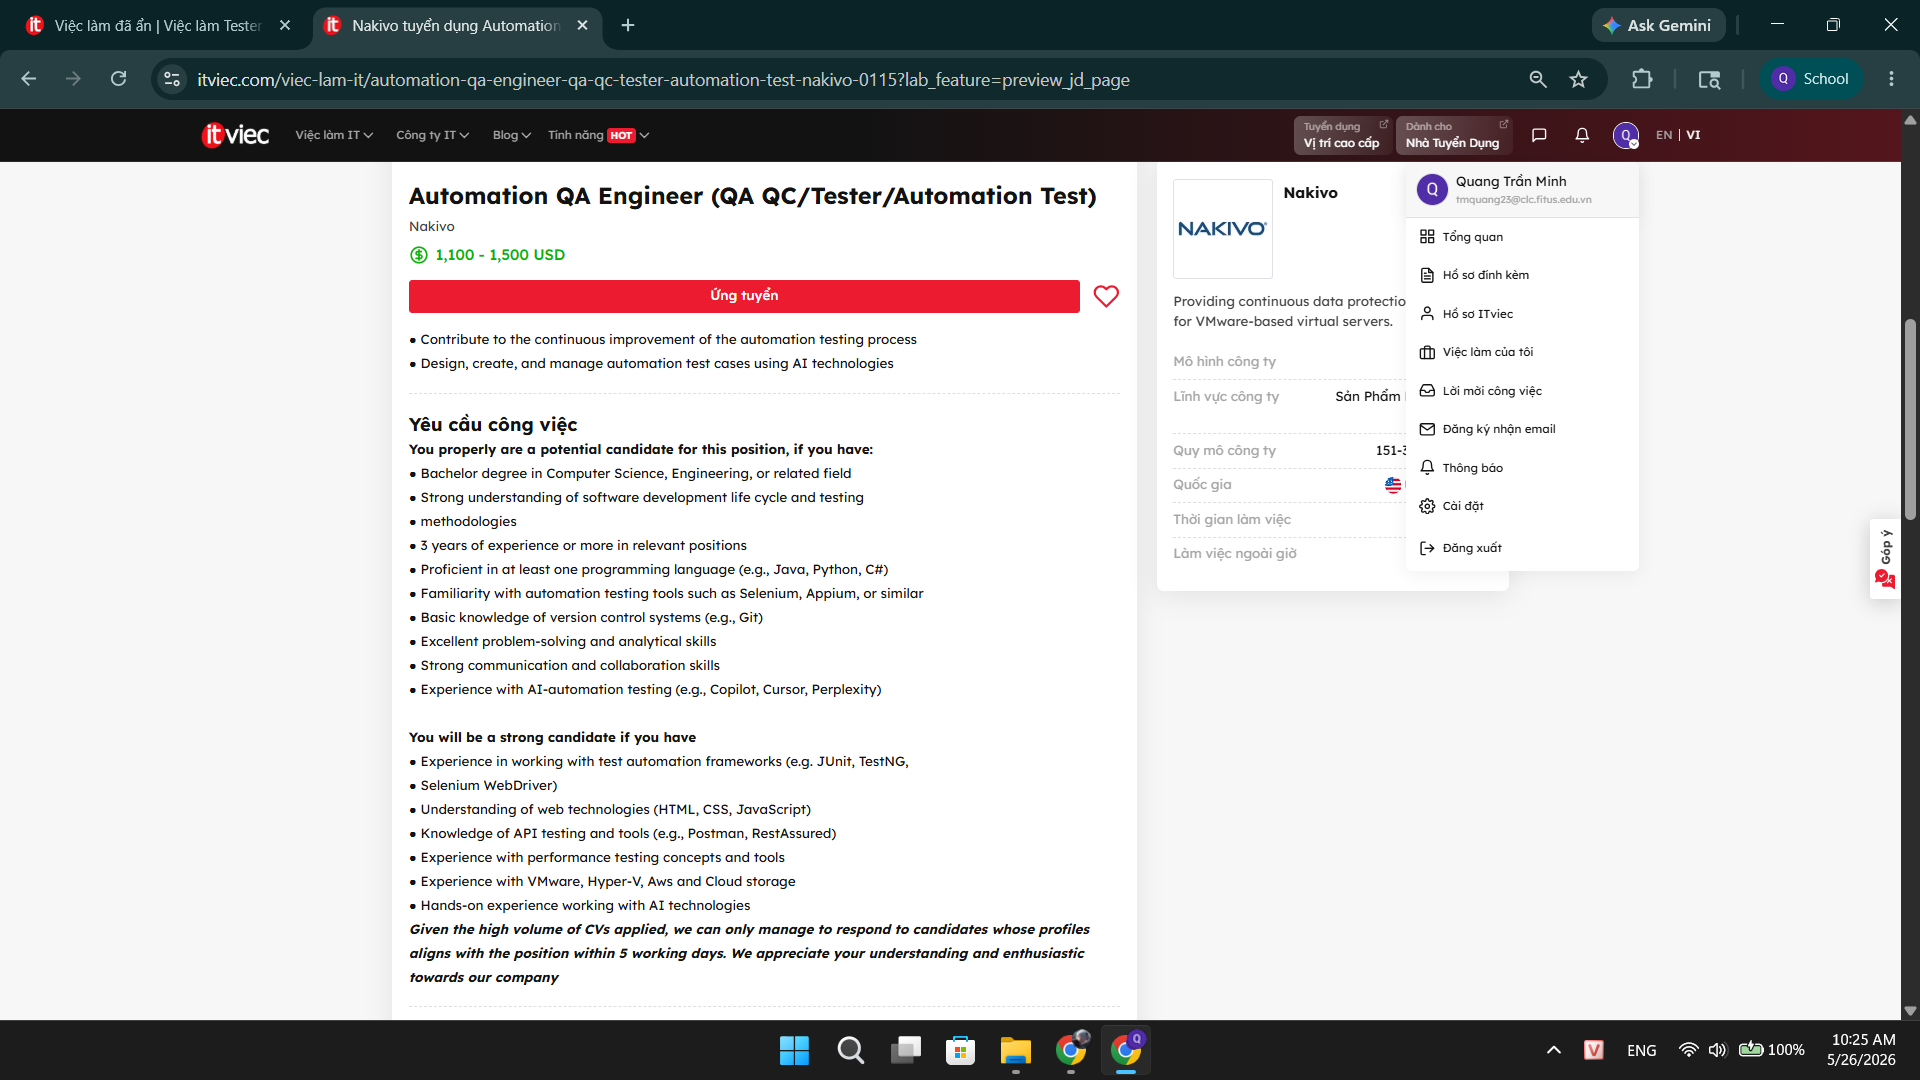
\includegraphics[scale=0.3]{pics_10_QA_QC_skilled/Automation_QA_Engineer_skilled.png}
\end{center}

\subsubsection{Mức lương}

Salary in range: 1,100 - 1,500 USD 

\subsubsection{Phân tích tác động của AI}

Với đề cập \textbf{"Design, create, and manage automation test cases using AI technologies."} trong mô tả , ta thấy được tác động mạnh mẽ của AI đối với công việc này khiến những kĩ năng của ứng viên về AI không còn đơn thuần là khuyến khích mà dường như nó là bắt buộc đối với các ứng viên. Bên cạnh đó, việc yêu cầu ứng viên có kinh nghiệm trong việc kiểm thử bằng AI như (Copilot, Cursor, Perplexity,...) đòi hỏi họ phải chuyển từ tư duy “tạo script tự động thủ công” sang “kết hợp với AI để tự động tạo, duy trì và cải tiến bộ test” nhằm tối ưu hóa công việc cũng như là đem đến kết quả tốt hơn.

\subsection{Tester (QA QC, Jira, Selenium, API)} 

\subsubsection{Đường dẫn công việc}
\href{https://itviec.com/viec-lam-it/tester-qa-qc-jira-selenium-api-cong-ty-tnhh-phat-trien-va-chuyen-giao-phan-mem-dtsoft-2350?lab_feature=preview_jd_page}{Tester (QA QC, Jira, Selenium, API) Link}

\subsubsection{Ảnh chụp màn hình công việc}
\begin{center}
    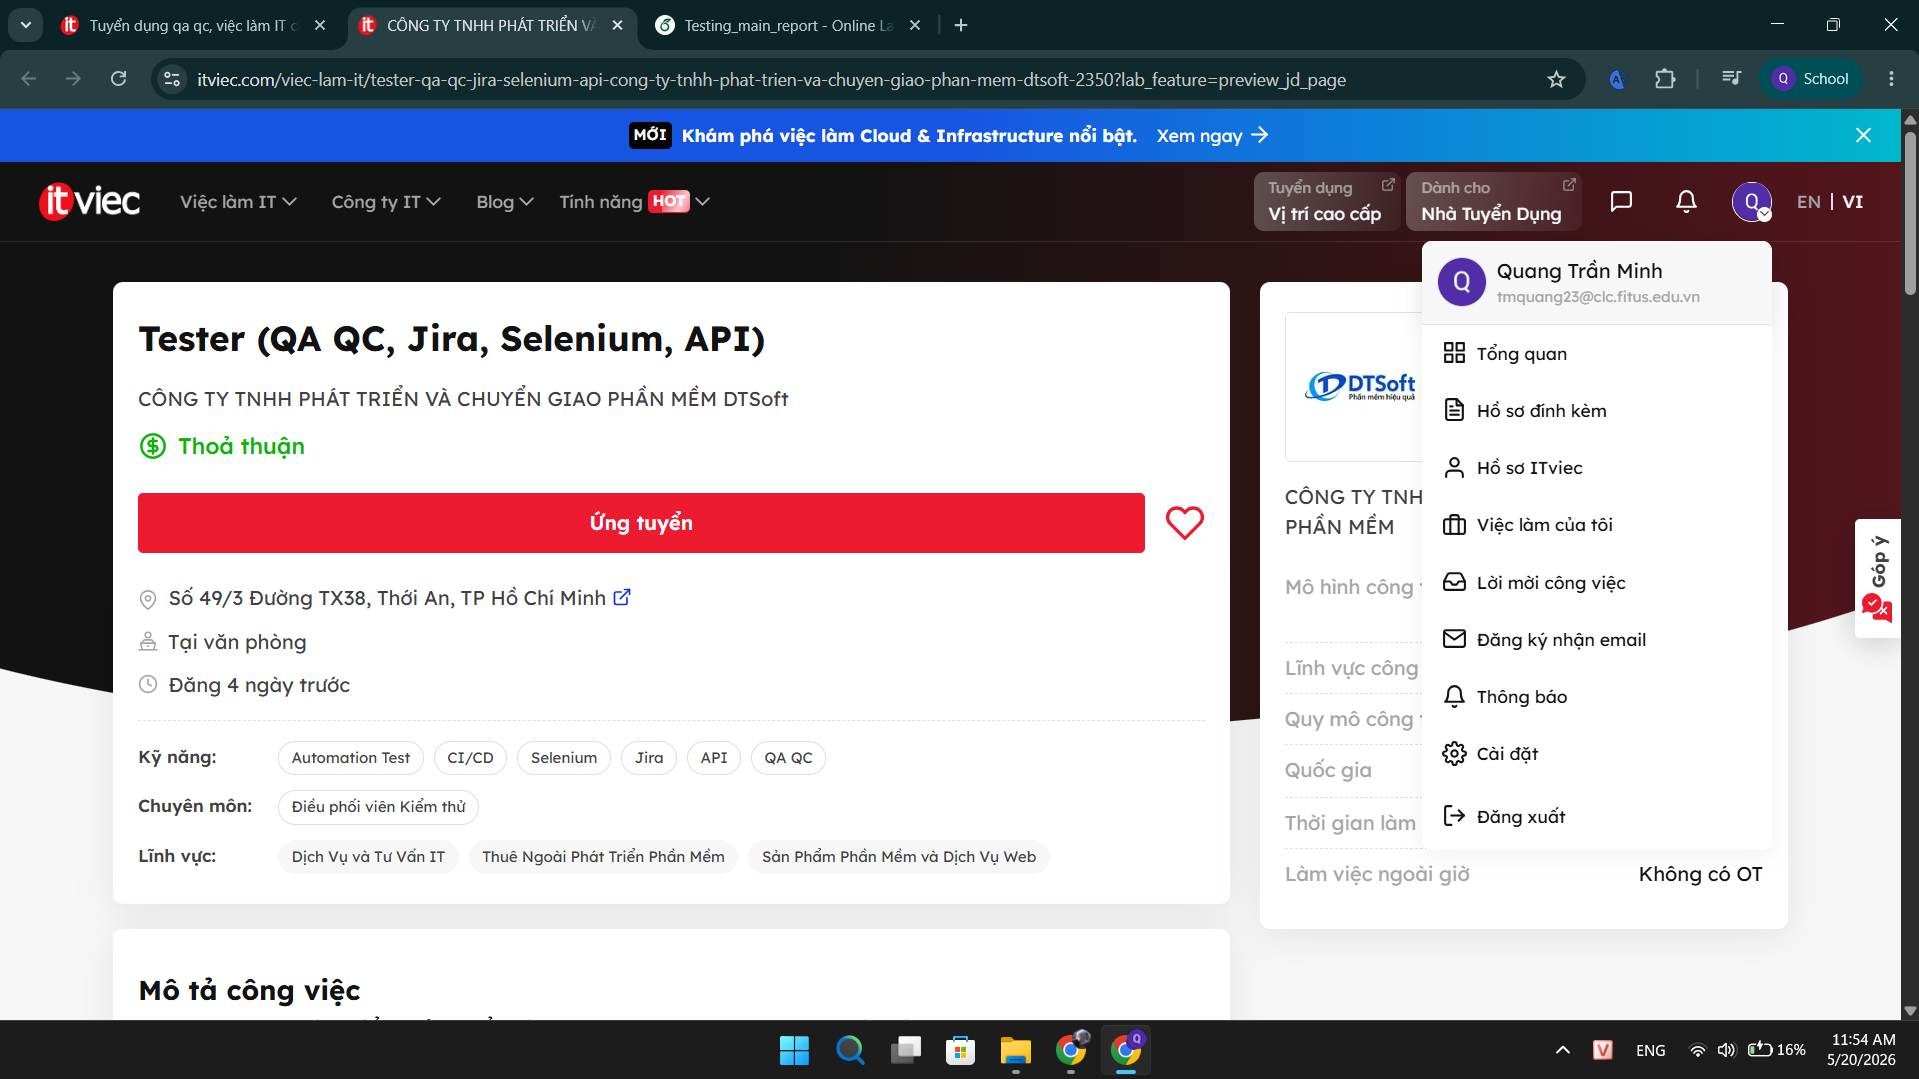
\includegraphics[scale=0.3]{pics_10_QA_QC/Tester (QA QC, Jira, Selenium, API).png}
\end{center}

\subsubsection{Mô tả công việc}
\begin{center}
    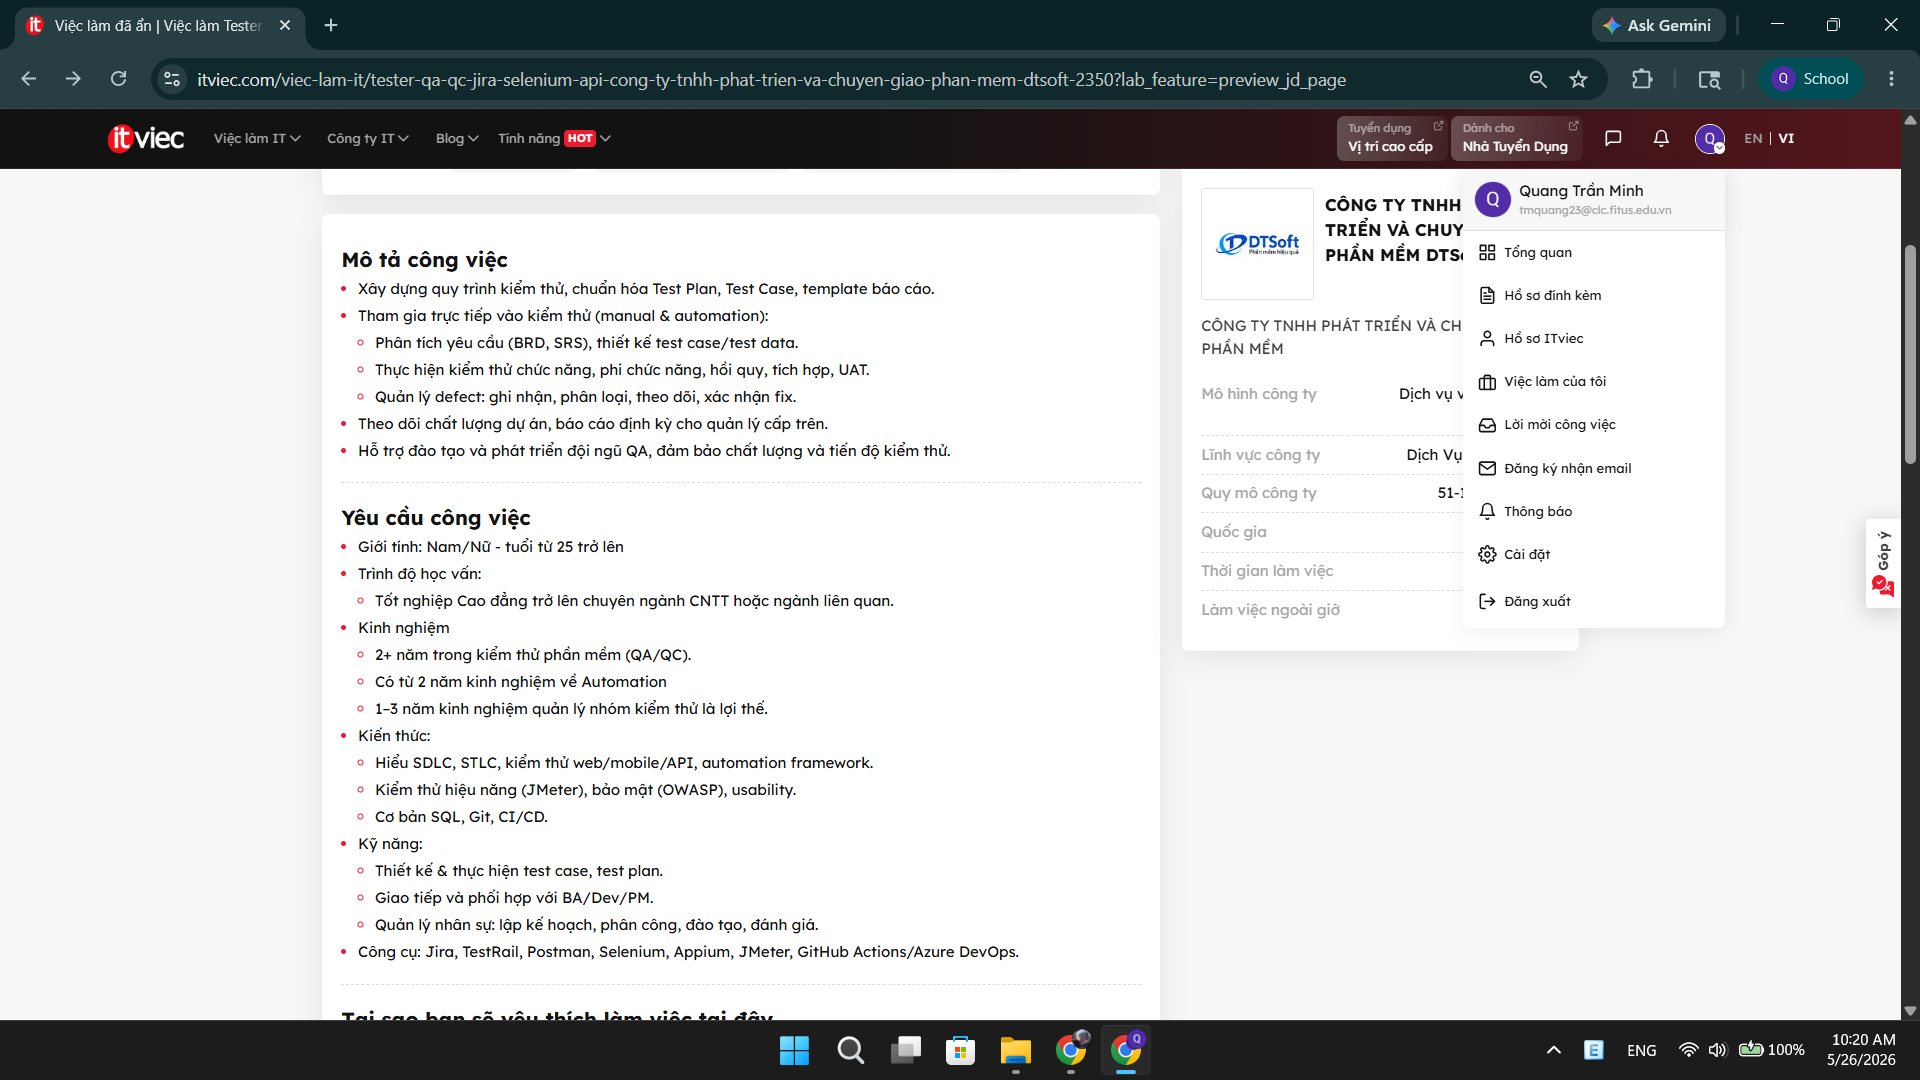
\includegraphics[scale=0.3]{pics_10_QA_QC_des/Tester_des.png}
\end{center}

\subsubsection{Các kĩ năng yêu cầu}

\begin{center}
    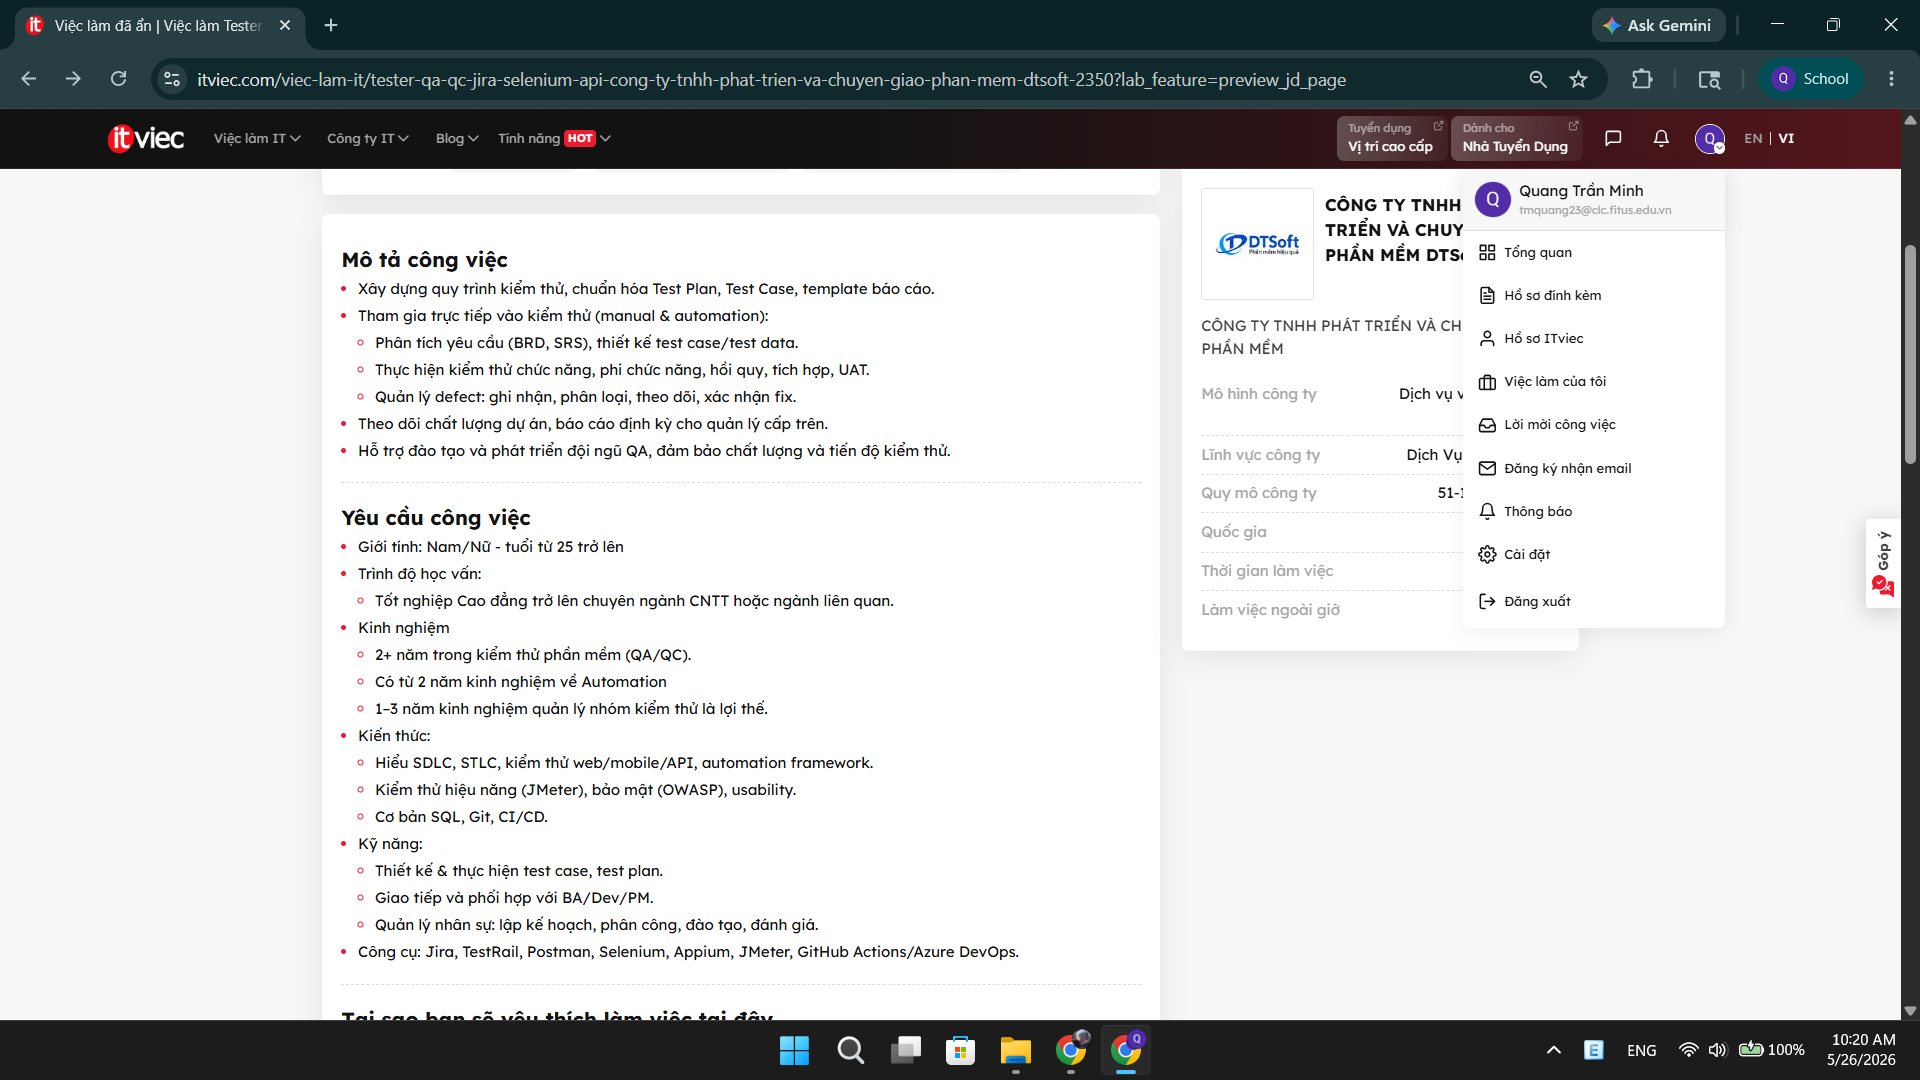
\includegraphics[scale=0.3]{pics_10_QA_QC_skilled/Tester_skilled.png}
\end{center}

\subsubsection{Mức lương}

Mức lương thỏa thuận.

\subsubsection{Phân tích tác động của AI}

Từ những mô tả cũng như yêu cầu kĩ năng của công việc, AI sẽ tác động mạnh mẽ đến các tác vụ thủ công như: \textbf{thiết kế test case/test data , quản lý defect,...} điều này đánh động mạnh mẽ đối với các ứng viên đáp ứng yêu cầu \textbf{ít nhất 2 năm kinh nghiệm về Automation} rằng họ cần có sự hợp tác với AI để làm việc một cách tối ưu và hiệu quả hơn. Bên cạnh đó, với sự vắng mặt của \textbf{AI-powered testing} cũng như \textbf{sử dụng công cụ AI} trong mô tả công việc đã phản ánh rõ sự lạc hậu của công ty đối với xu hướng trên thị trường và nguy cơ làm mất giá trị kỹ sư QA

\subsection{Senior/ Leader QA Tester (ERP, API, SQL, NoSQL)} 

\subsubsection{Đường dẫn công việc}
\href{https://itviec.com/viec-lam-it/senior-leader-qa-tester-erp-api-sql-nosql-ai-di-2153?lab_feature=similar_job}{Senior/ Leader QA Tester (ERP, API, SQL, NoSQL) Link}

\subsubsection{Ảnh chụp màn hình công việc}
\begin{center}
    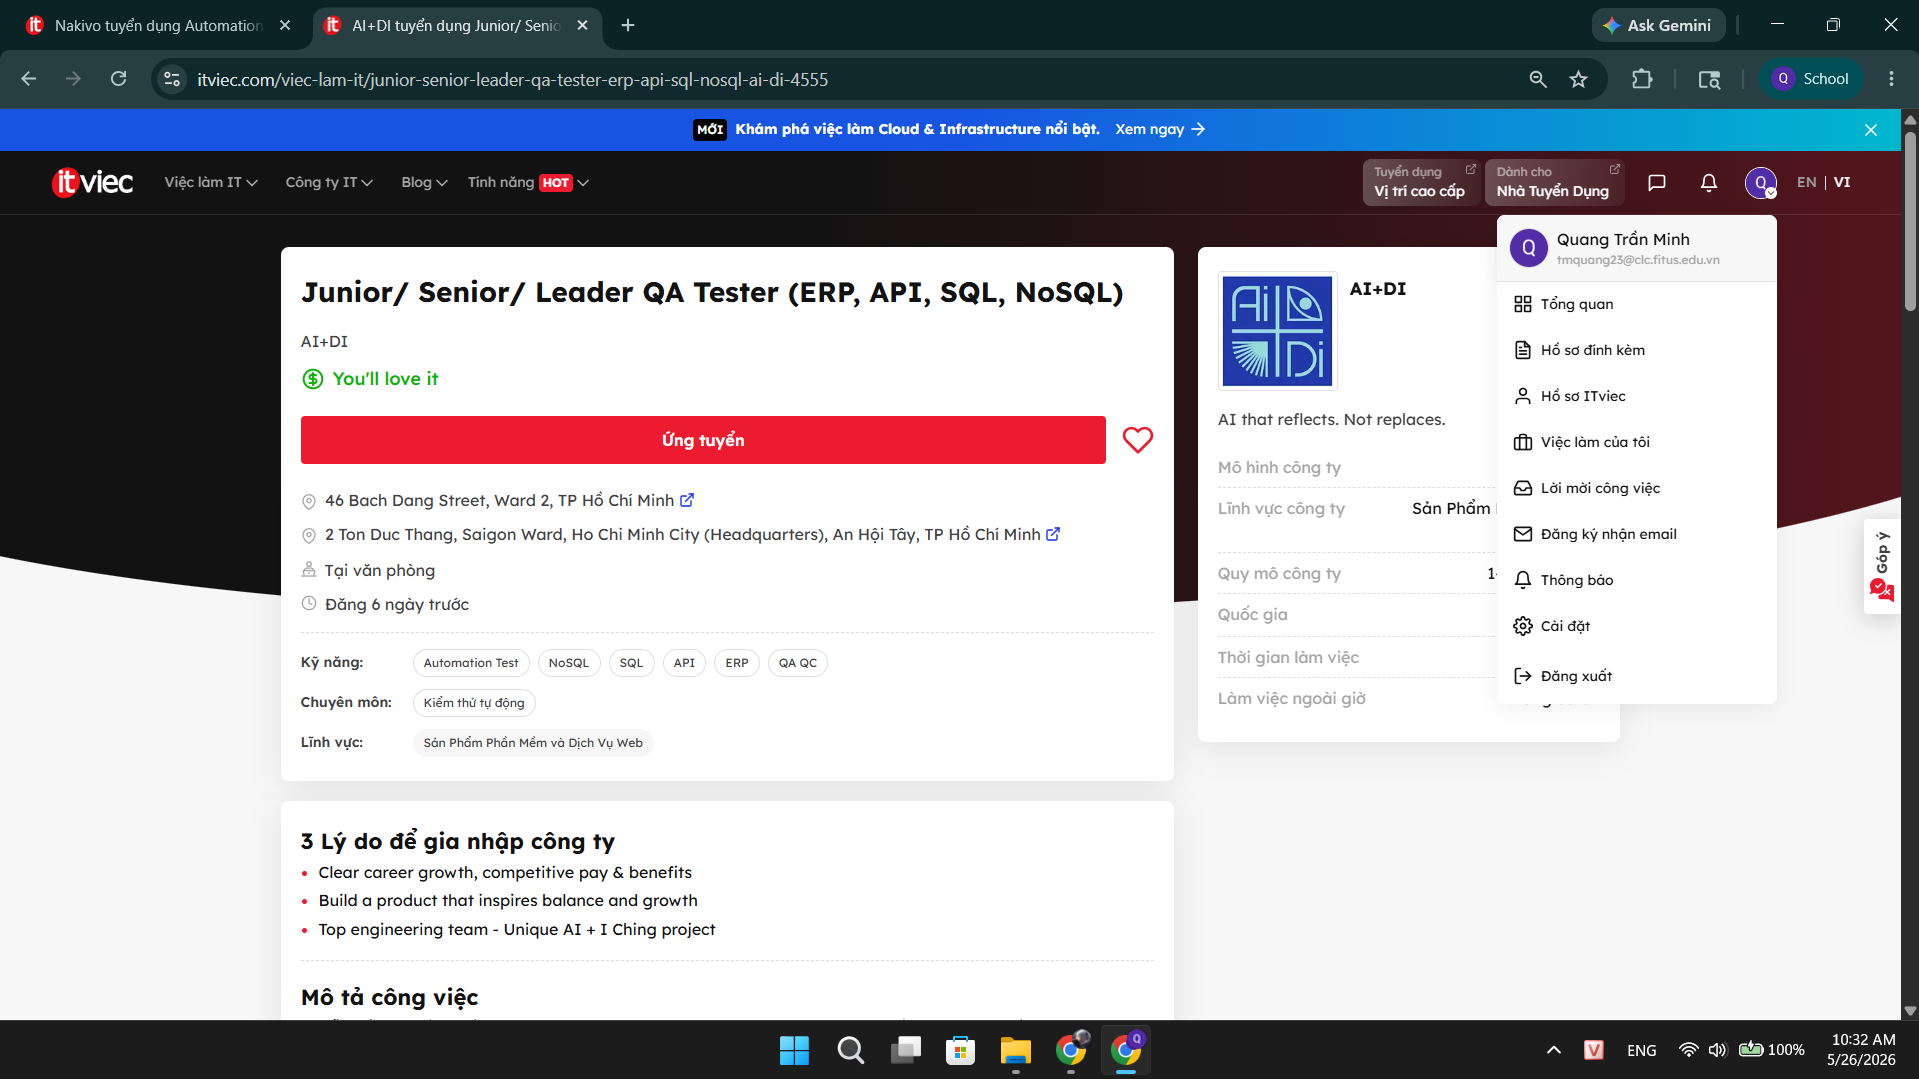
\includegraphics[scale=0.3]{pics_10_QA_QC/Senior Leader QA Tester (ERP, API, SQL, NoSQL).png}
\end{center}

\subsubsection{Mô tả công việc}
\begin{center}
    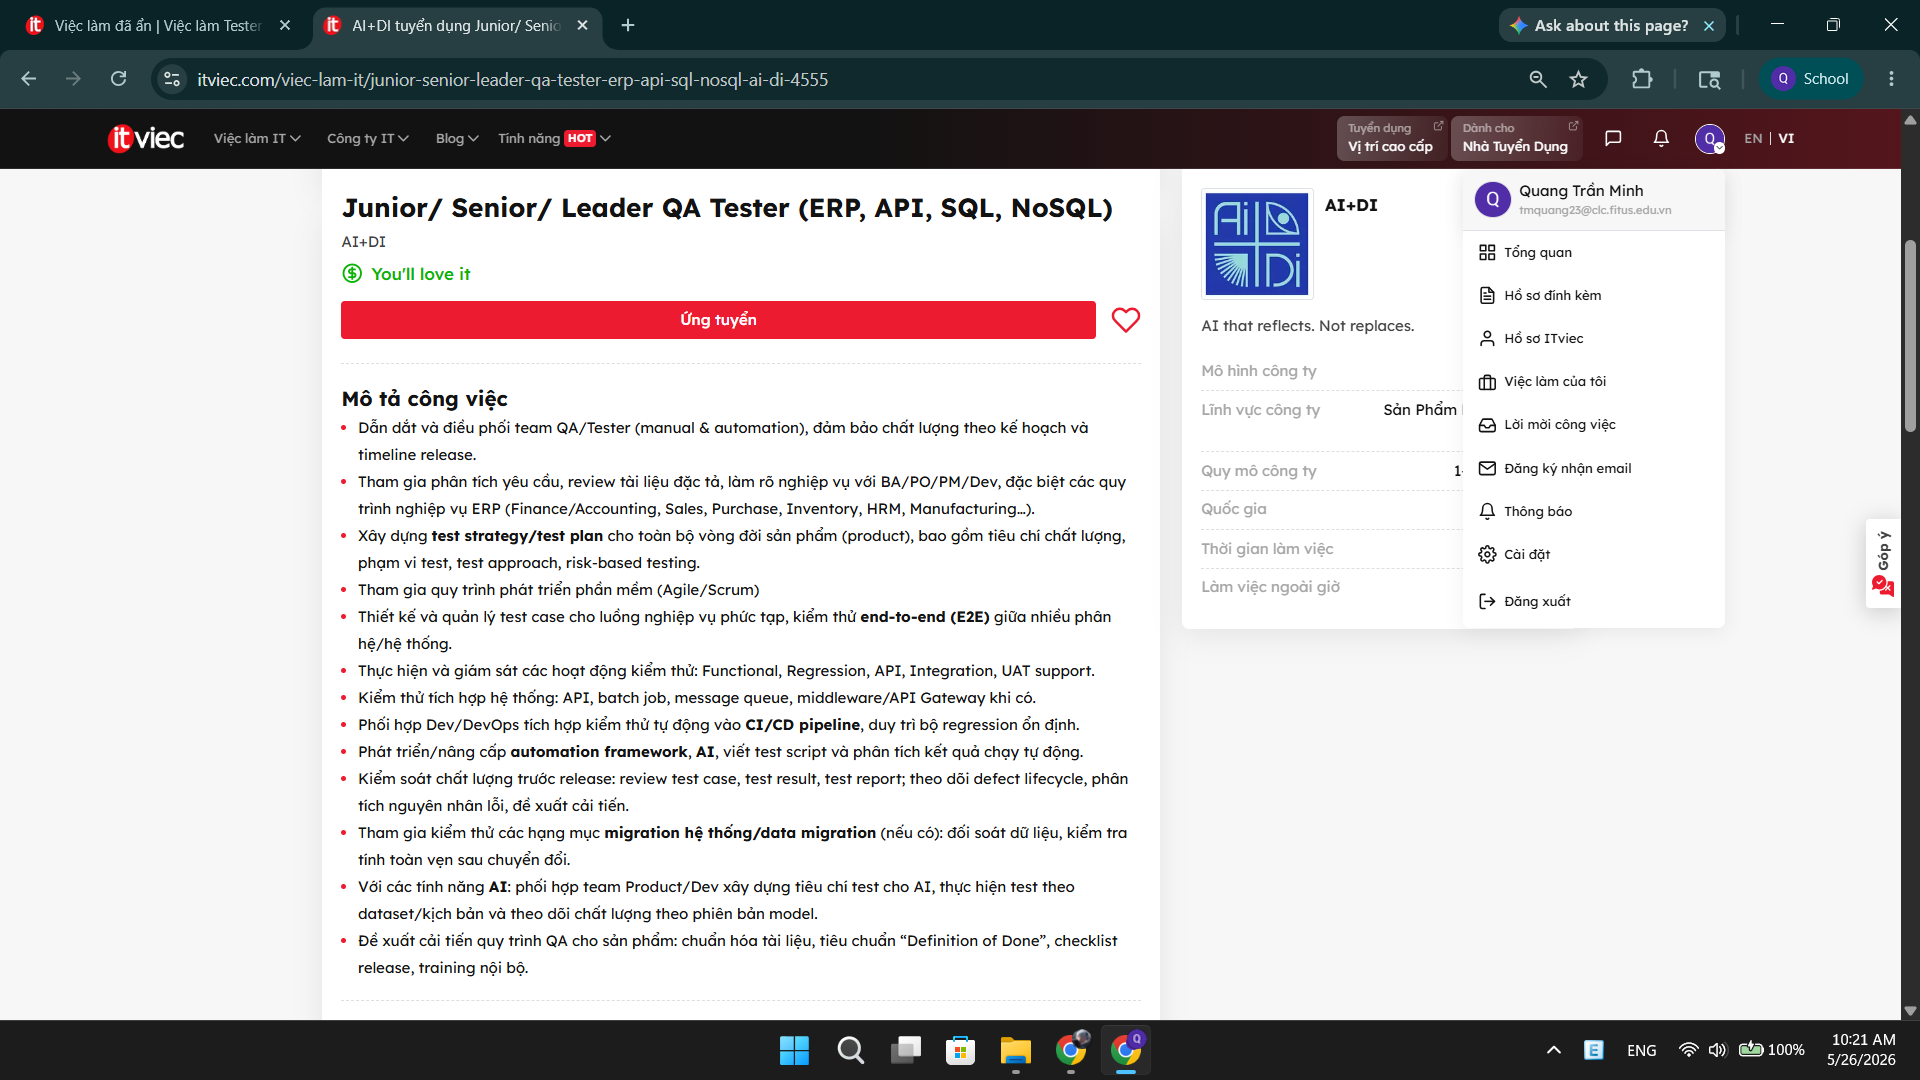
\includegraphics[scale=0.3]{pics_10_QA_QC_des/Senior_Leader_QA_Tester_des.png}
\end{center}

\subsubsection{Các kĩ năng yêu cầu}

\begin{center}
    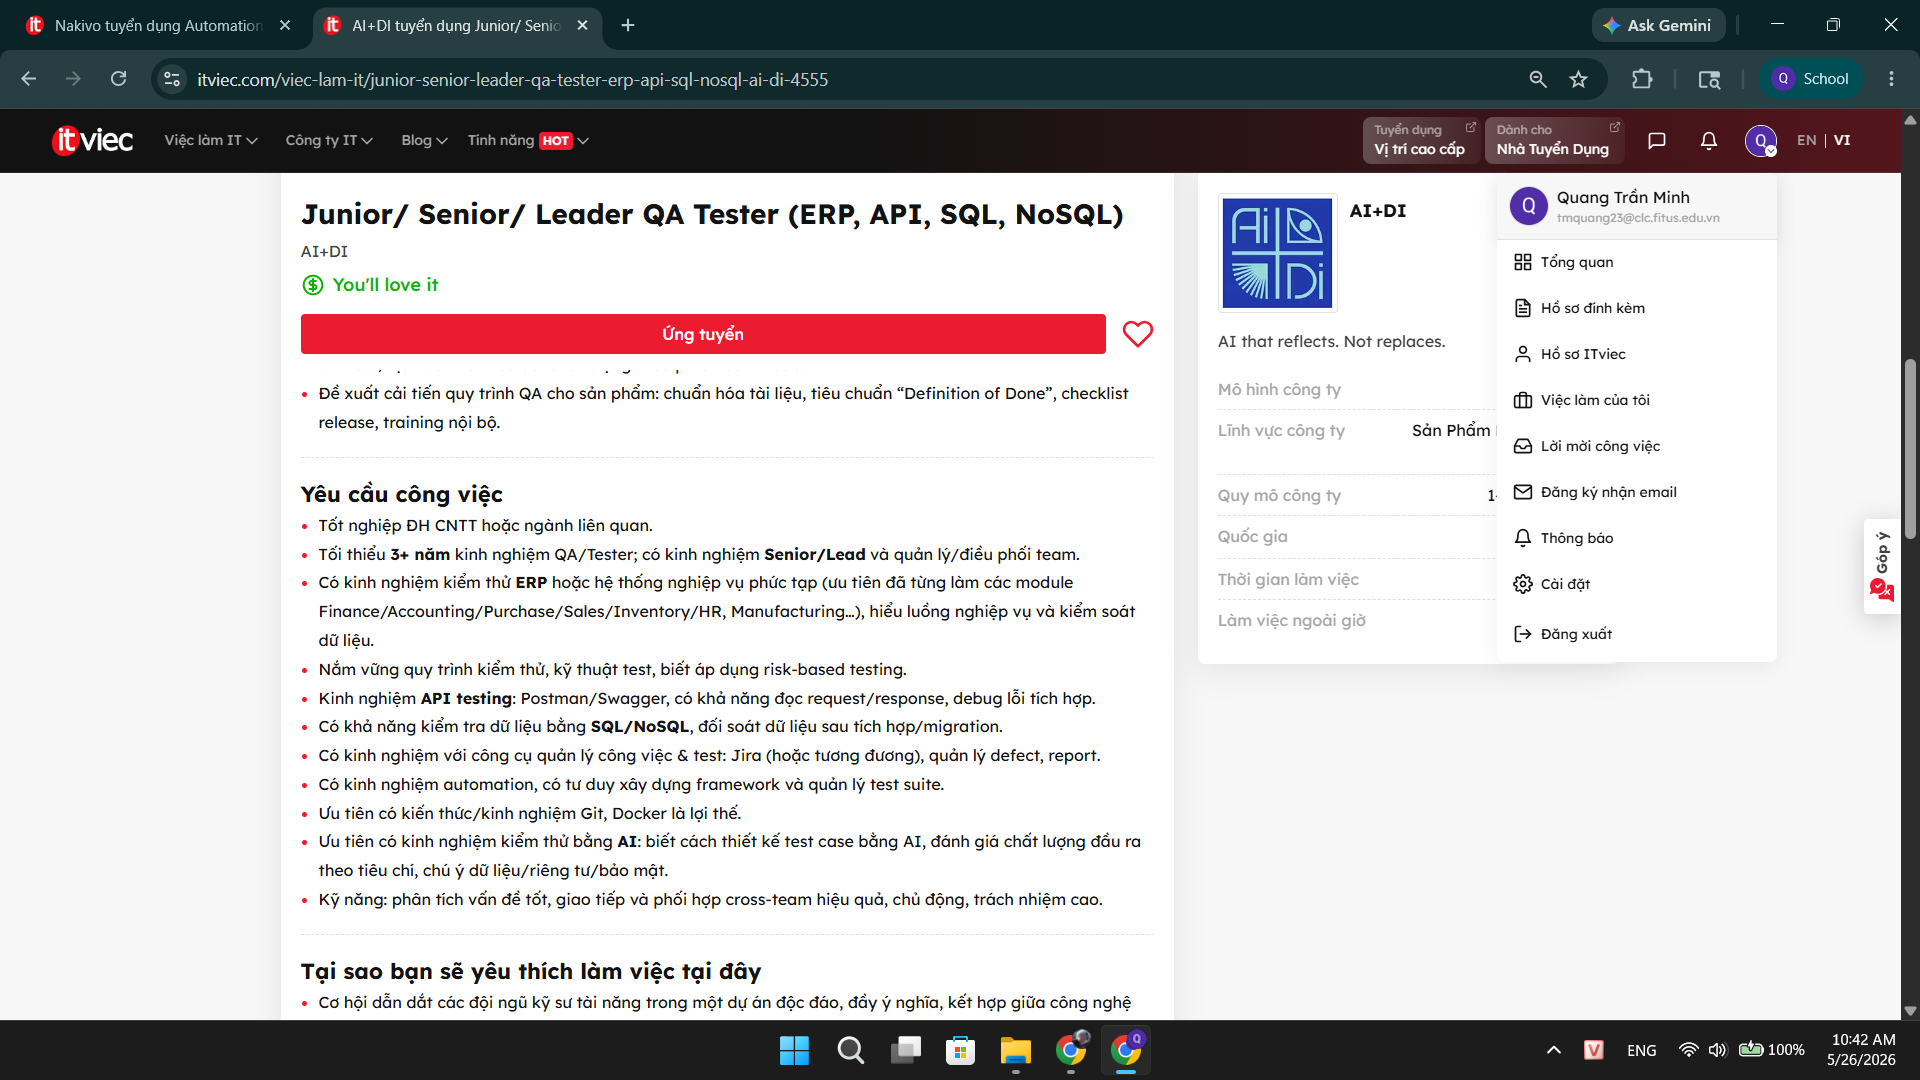
\includegraphics[scale=0.3]{pics_10_QA_QC_skilled/Senior_Leader_QA_Tester_skilled.png}
\end{center}

\subsubsection{Mức lương}

Mức lương nằm trong khoảng: 1,000 - 1,400 USD

\subsubsection{Phân tích tác động của AI}

AI có ảnh hưởng rất lớn đối với vị trí Junior/Senior/Leader QA Tester này khi công ty đề cập đến \textbf{"testing AI"} vào phần mô tả công việc chính, đòi hỏi Leader cần làm việc với Dev để xác định tiêu chí test cho AI, testing AI theo dataset và monitoring chất lượng AI qua các phiên bản model. Đây cũng chính là cơ hội tốt để làm việc trong môi trường QA chuyên nghiệp, nơi công ty đã chủ động áp dụng AI vào quy trình kiểm thử.

\subsection{Automation Tester (QA QC)} 

\subsubsection{Đường dẫn công việc}
\href{https://itviec.com/viec-lam-it/automation-tester-qa-qc-mercatus-4125?lab_feature=preview_jd_page}{Automation Tester ( QA QC) Link}

\subsubsection{Ảnh chụp màn hình công việc}
\begin{center}
    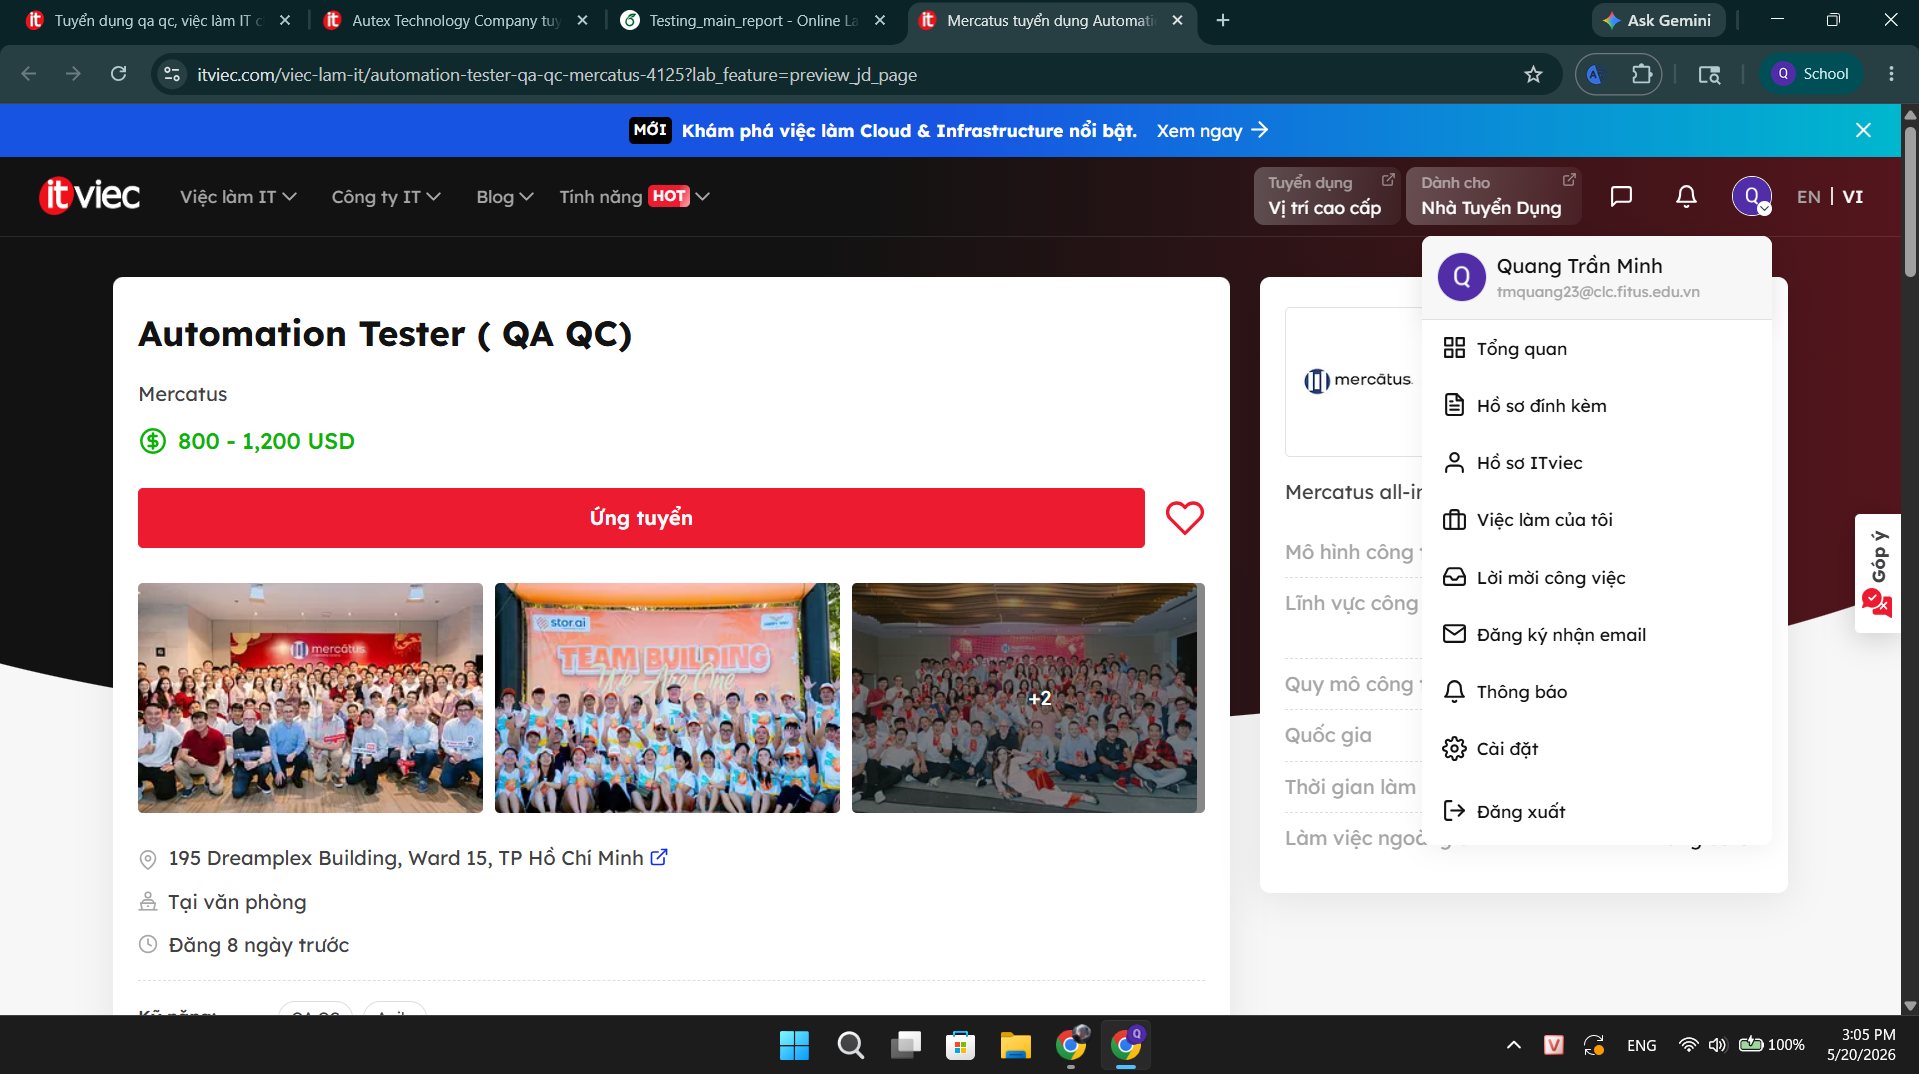
\includegraphics[scale=0.3]{pics_10_QA_QC/Automation Tester ( QA QC).png}
\end{center}

\subsubsection{Mô tả công việc}
\begin{center}
    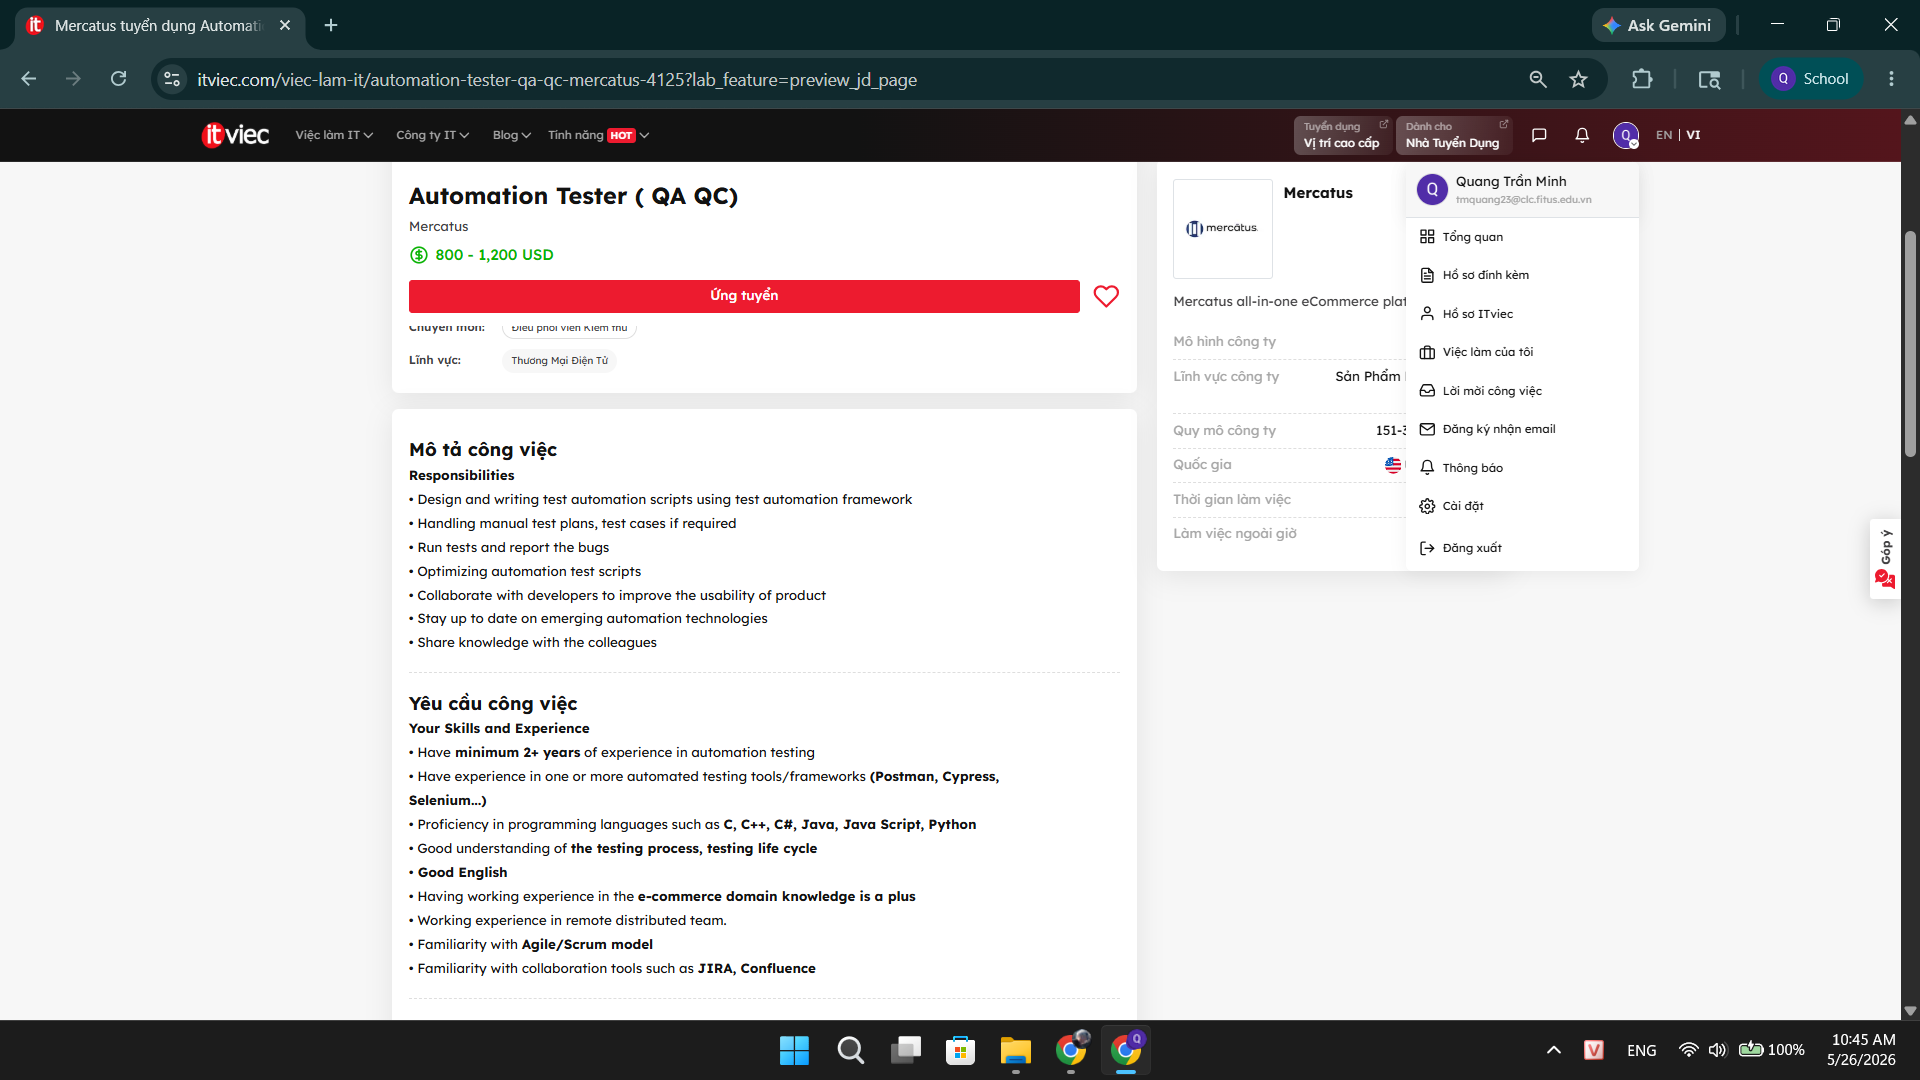
\includegraphics[scale=0.3]{pics_10_QA_QC_des/Automation_Tester_des.png}
\end{center}

\subsubsection{Các kĩ năng yêu cầu}

\begin{center}
    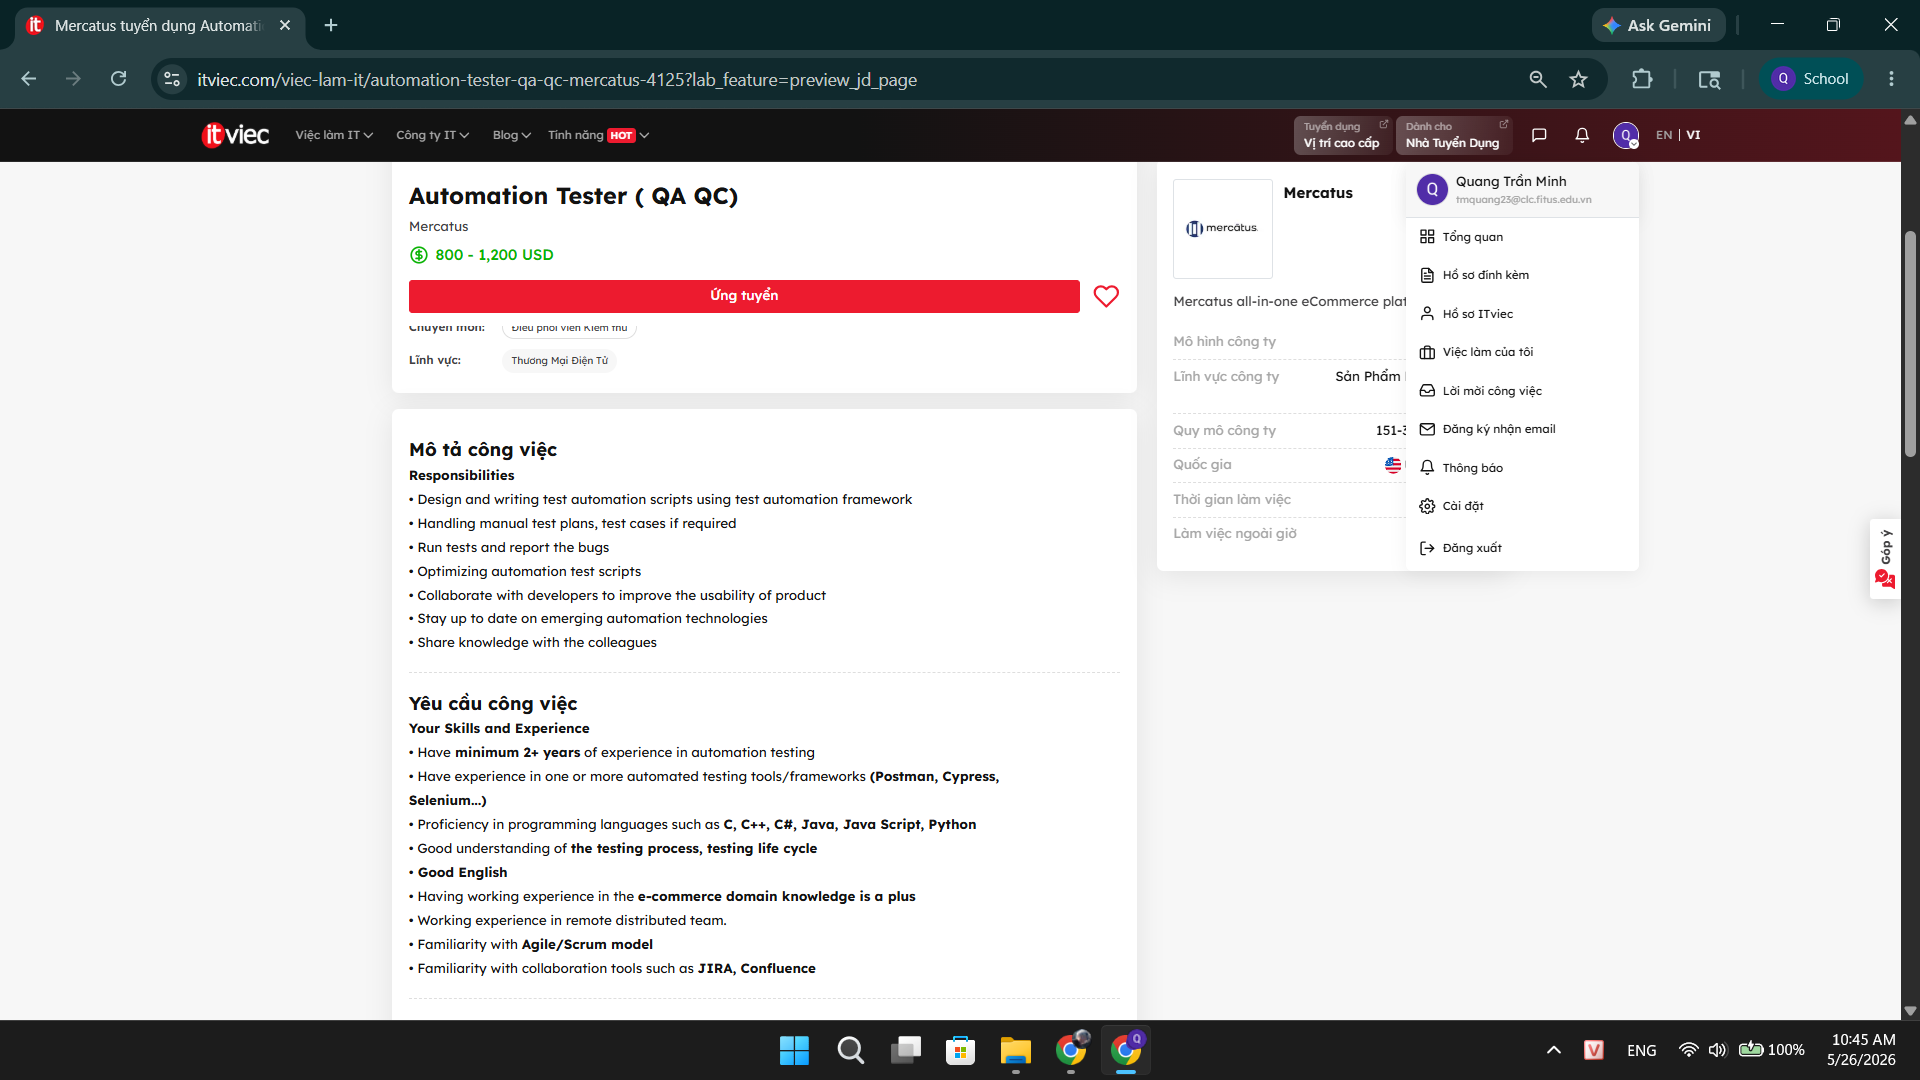
\includegraphics[scale=0.3]{pics_10_QA_QC_skilled/Automation_Tester_skilled.png}
\end{center}

\subsubsection{Mức lương}

Salary in range: 800 - 1,200 USD

\subsubsection{Phân tích tác động của AI}

Tác động của AI lên vị trí Automation Tester này được thể hiện thông qua yêu cầu \textbf{"Stay up to date on emerging automation technologies"} trong khi mô tả hiện tại không hề nhắc tới bất kỳ công nghệ nào liên quan đến việc sử dụng AI trong việc kiểm thử phần mềm (như self-healing locators, AI-assisted test generation, hoặc các công cụ như Copilot, Cursor) khiến cho vị trí này rất dễ trở nên lỗi thời do chỉ phụ thuộc vào Selenium, Cypress và các framework automation khác. Nếu không chủ động đưa AI vào việc viết automation script, người kỹ sư QA ở vị trí này rất dễ mất giá trị do xu hướng mới của thị trường.

\subsection{QC Engineer (Tester/QA QC) for Web} 

\subsubsection{Đường dẫn công việc}
\href{https://itviec.com/viec-lam-it/qc-engineer-tester-qa-qc-for-web-up-to-1500-evolus-planv-5225?lab_feature=similar_job}{QC Engineer (Tester/QA QC) for Web Link}

\subsubsection{Ảnh chụp màn hình công việc}
\begin{center}
    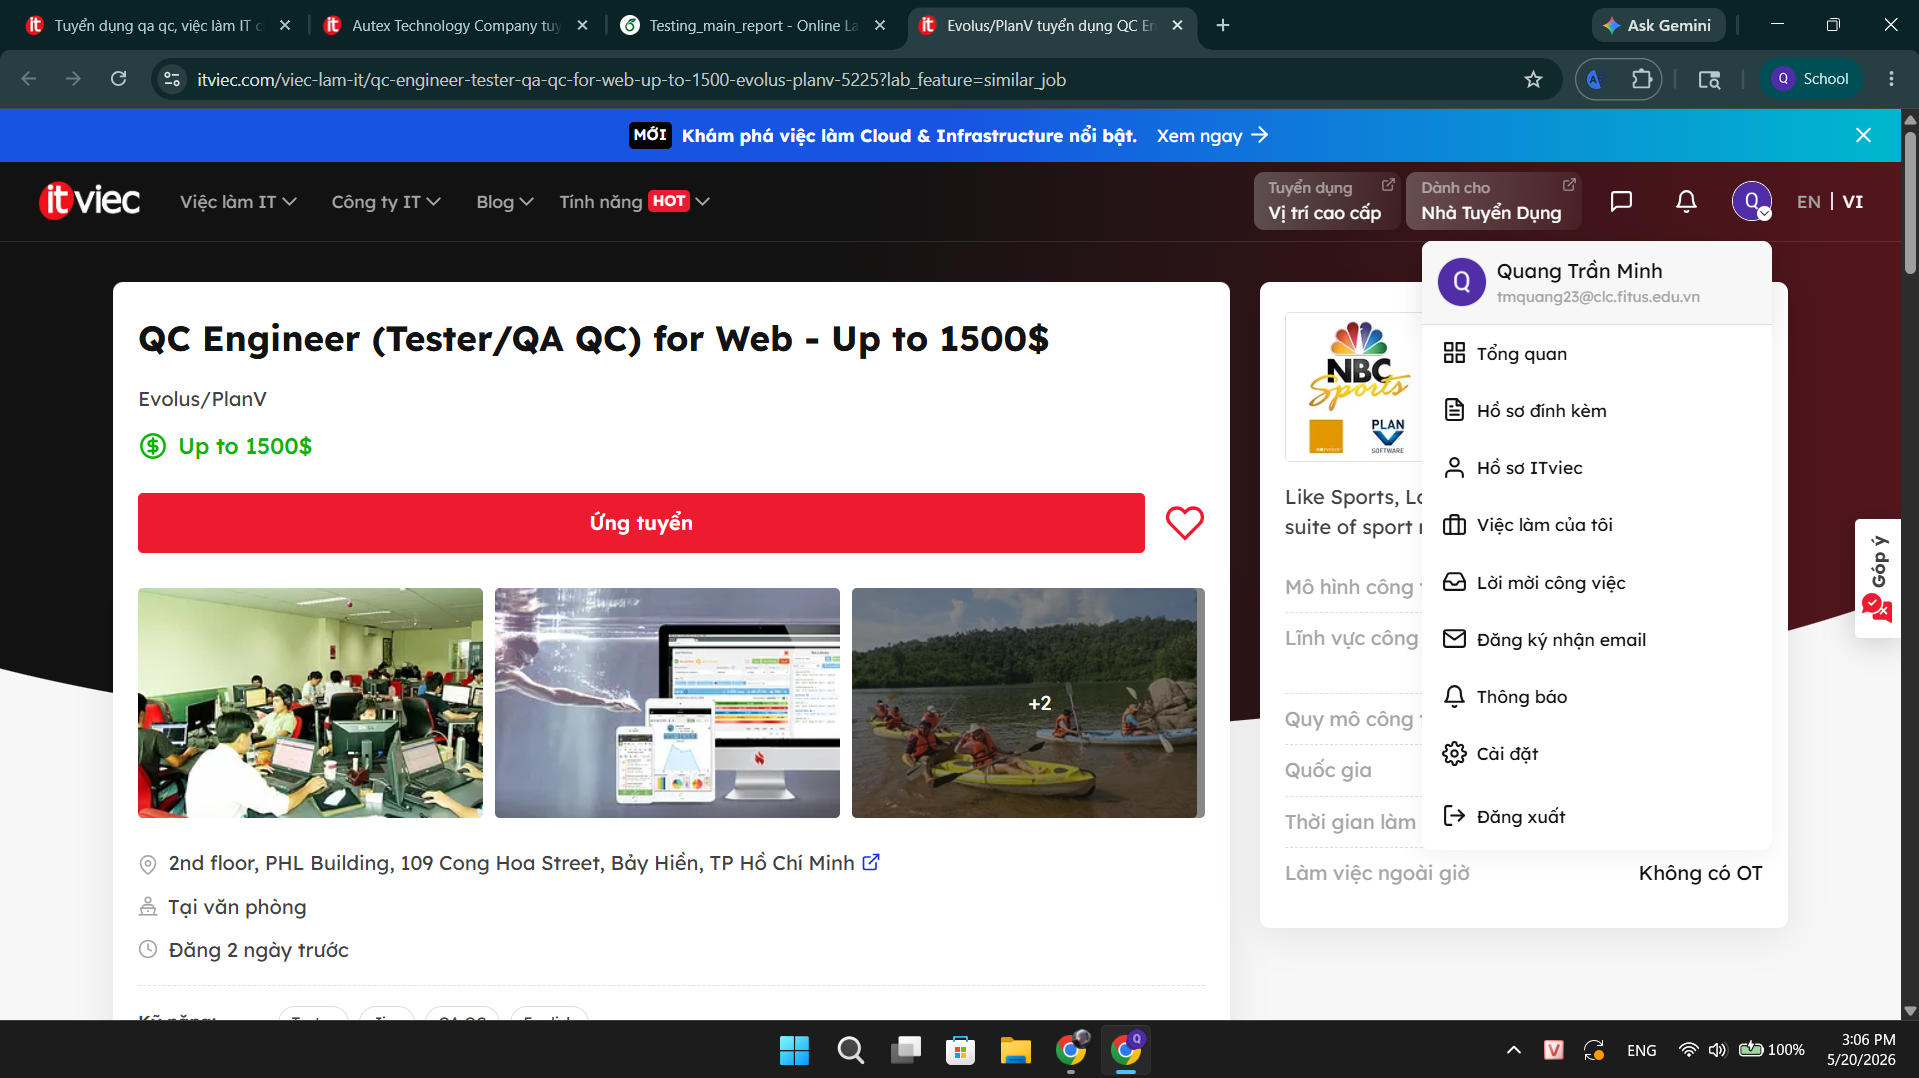
\includegraphics[scale=0.3]{pics_10_QA_QC/QC Engineer (Tester QA QC) for Web.png}
\end{center}

\subsubsection{Mô tả công việc}
\begin{center}
    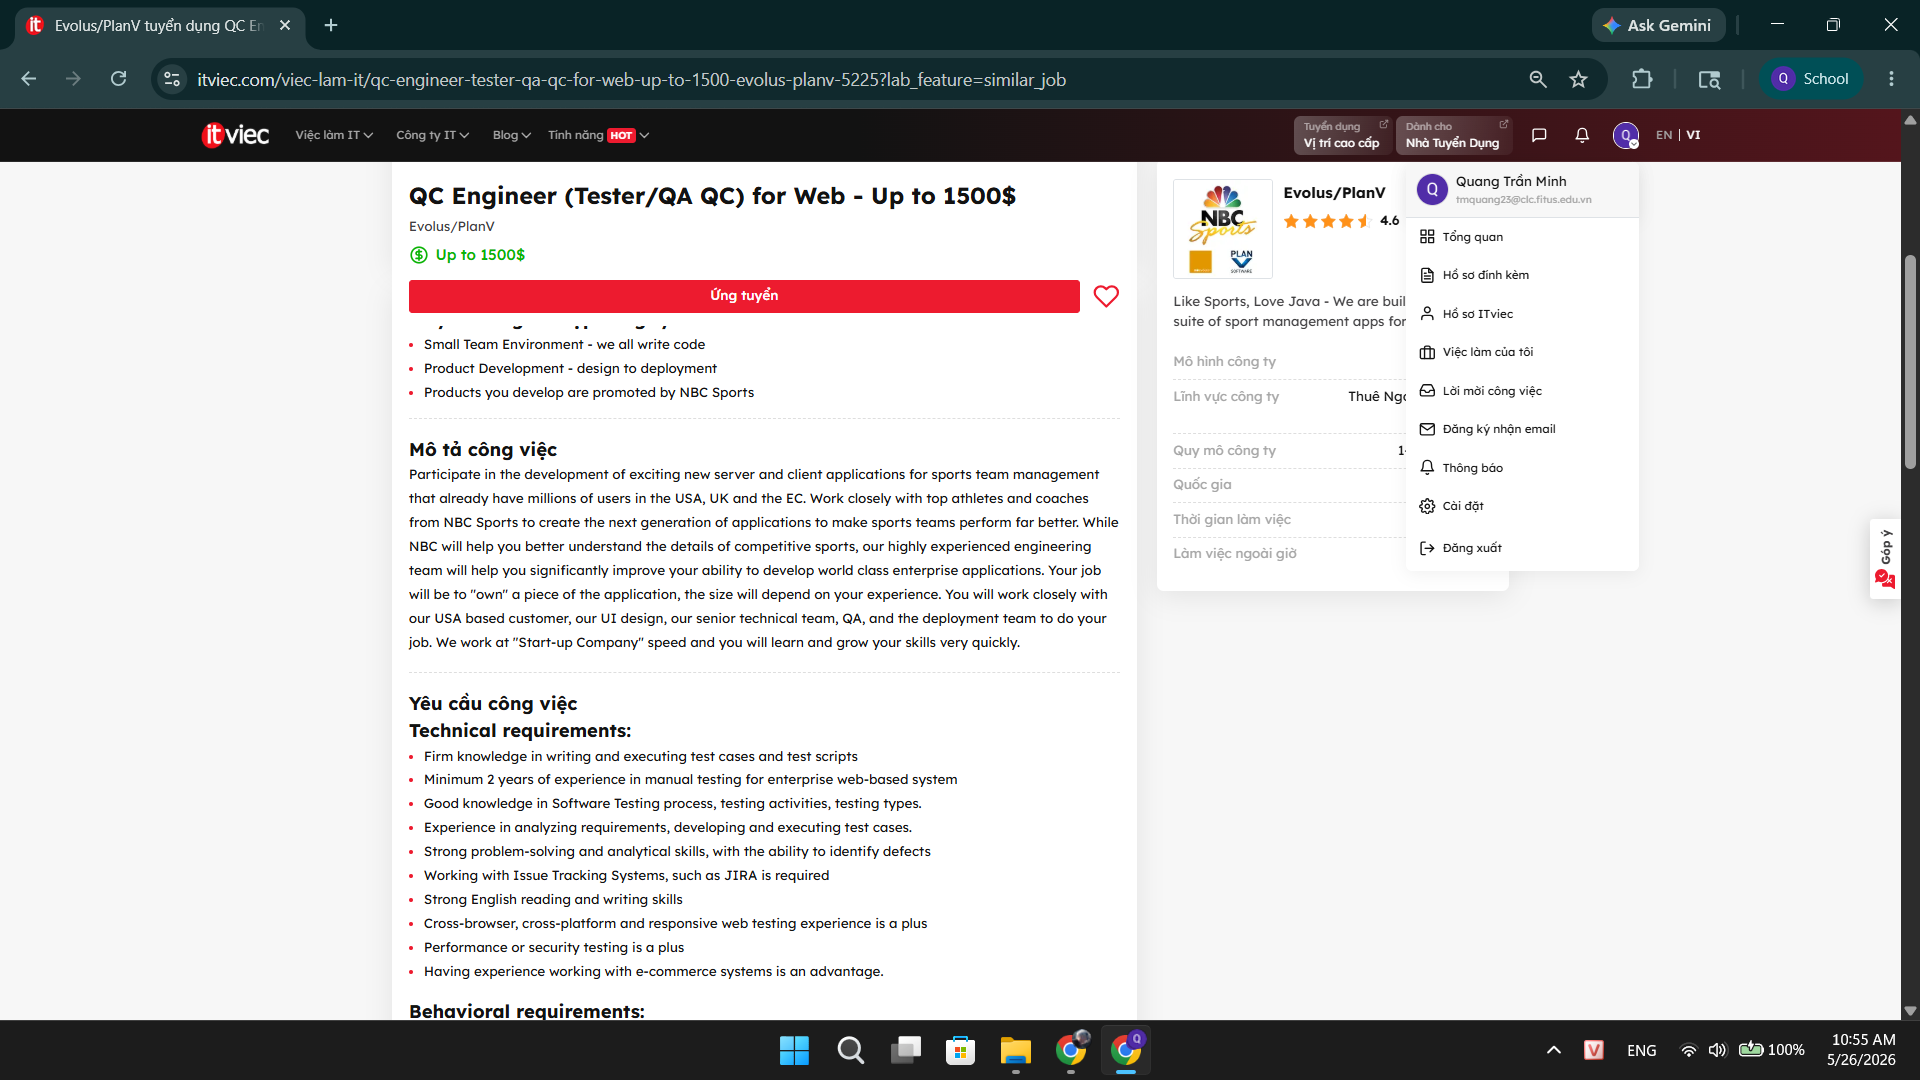
\includegraphics[scale=0.3]{pics_10_QA_QC_des/QC_Engineer_des.png}
\end{center}
\subsubsection{Các kĩ năng yêu cầu}

\begin{center}
    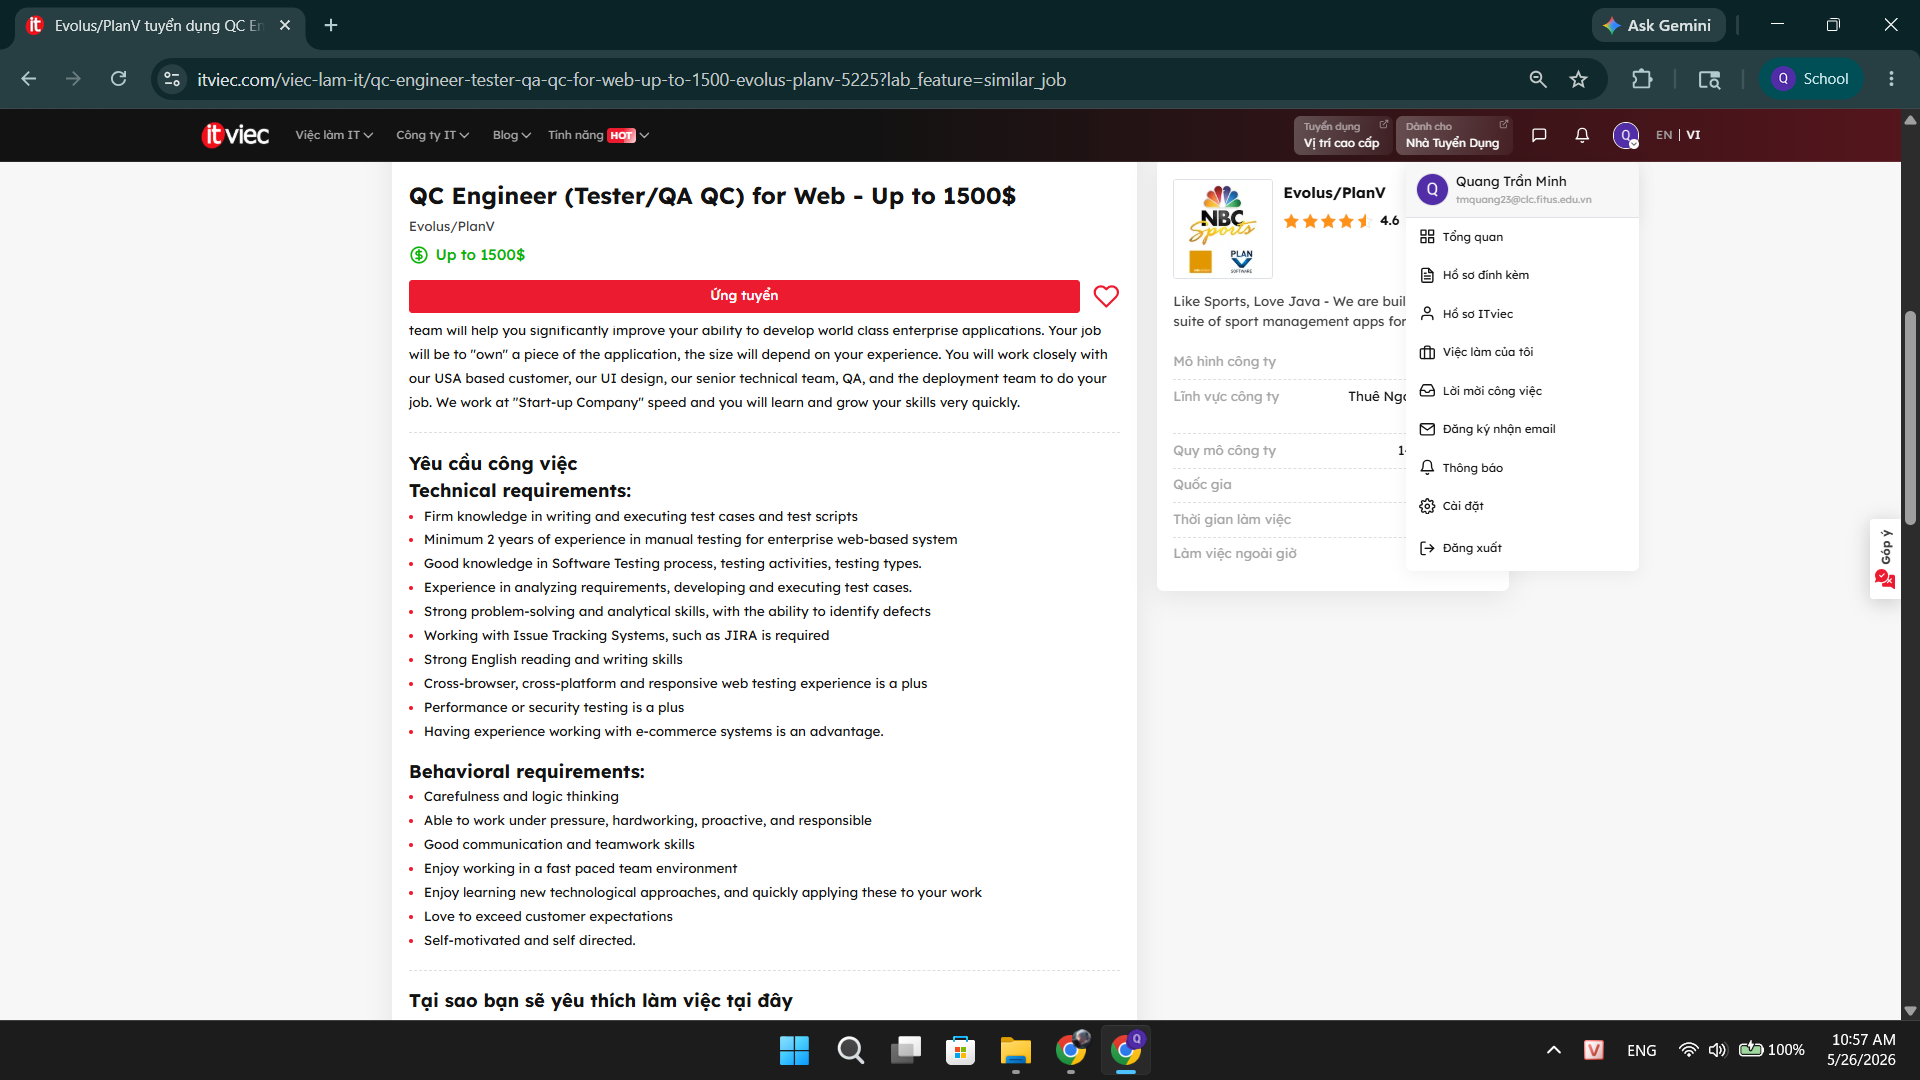
\includegraphics[scale=0.3]{pics_10_QA_QC_skilled/QC_Engineer_skilled.png}
\end{center}

\subsubsection{Mức lương}

Salary up to 1,500 USD

\subsubsection{Phân tích tác động của AI}

Tác động của AI sẽ ảnh hưởng tới công việc QC Engineer ở điểm này vì công việc đòi hỏi \textbf{"Enjoy learning new technological approaches, and quickly applying these to your work"}, nhưng thông tin về kỹ năng lại không đề cập gì đến automation hay AI, mà chỉ tập trung vào manual testing trên web. Điều này tạo nên mối lo ngại về tương lai của công việc này khi không phải do không muốn học hỏi mà vì công ty không định hướng cho AI hay automation, QC engineer vẫn tiếp tục công việc thủ công của mình dẫn đến tỉ lệ cao bị thay thế sau này.

\subsection{Web3 QAQC} 

\subsubsection{Đường dẫn công việc}
\href{https://itviec.com/viec-lam-it/web3-qaqc-autex-technology-company-5027?lab_feature=preview_jd_page}{Web3 QAQC Link}

\subsubsection{Ảnh chụp màn hình công việc}
\begin{center}
    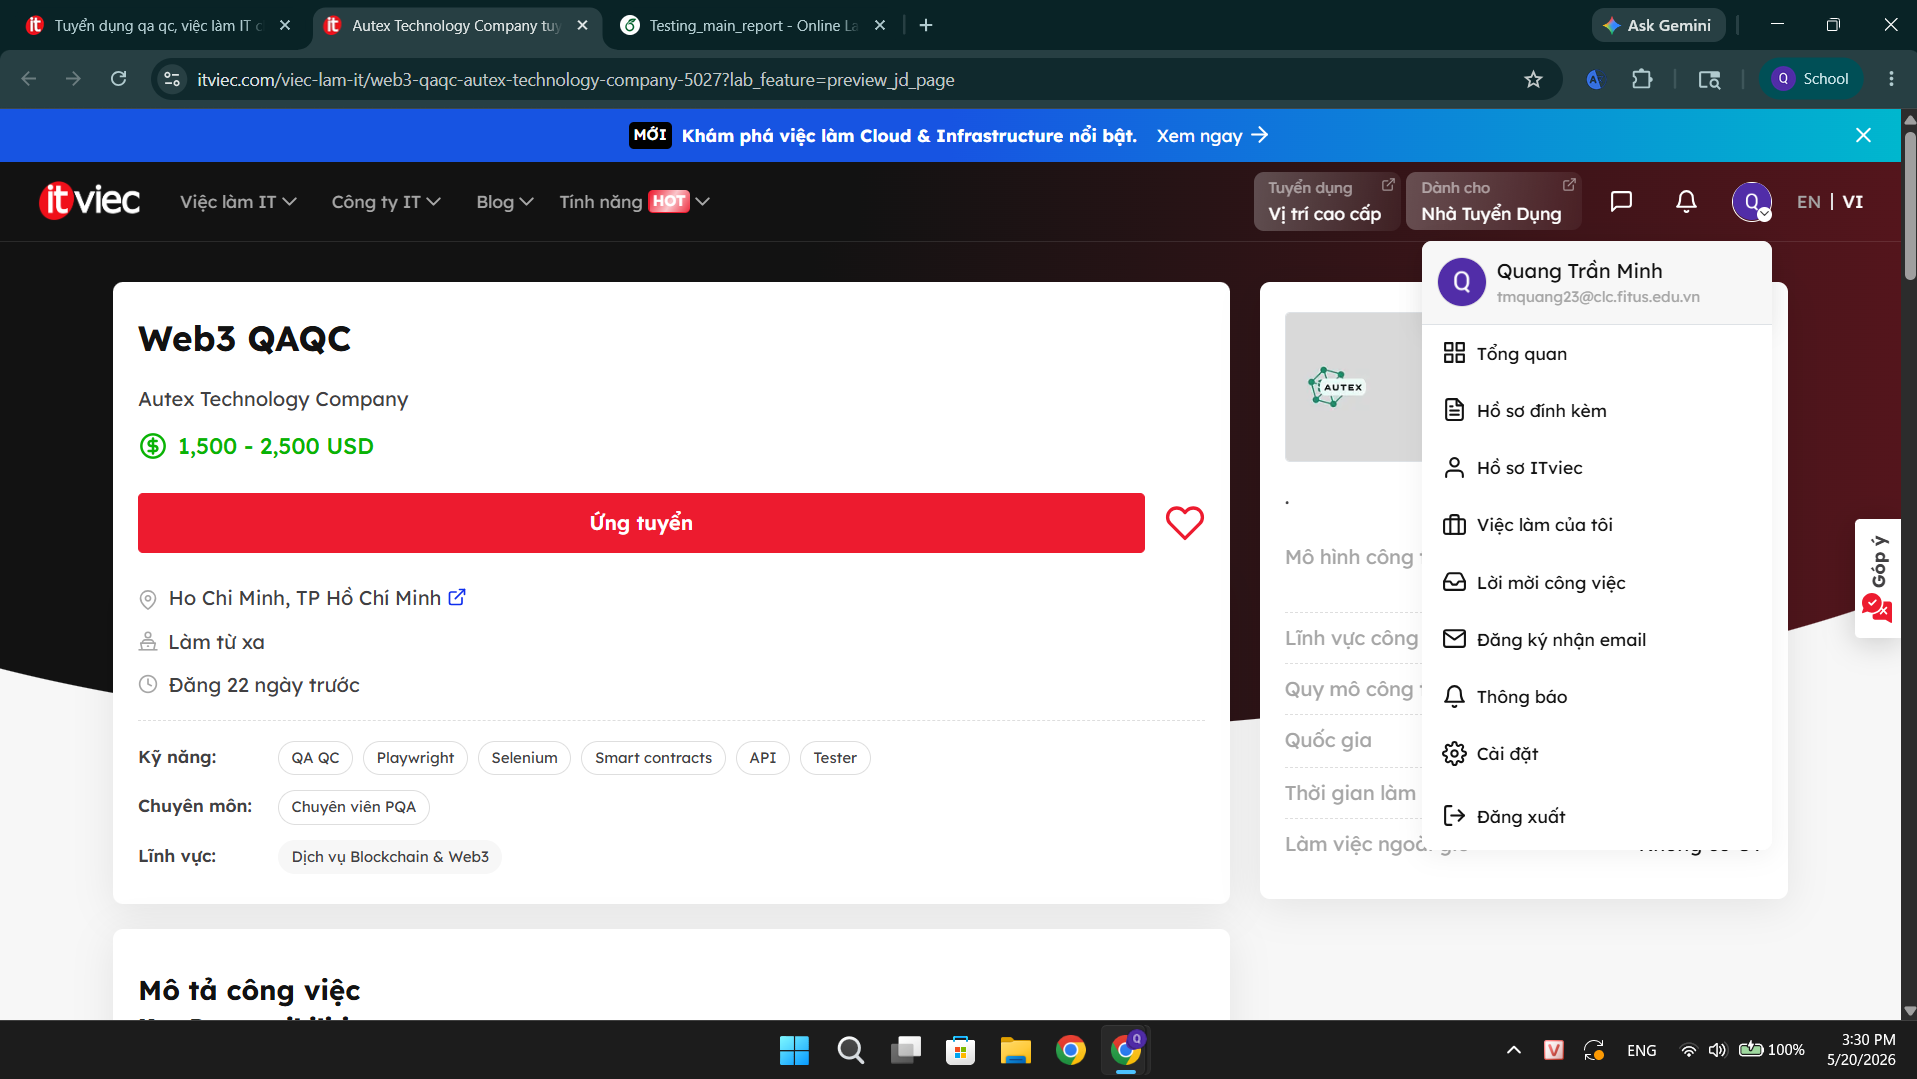
\includegraphics[scale=0.3]{pics_10_QA_QC/Web3 QAQC.png}
\end{center}

\subsubsection{Mô tả công việc}
\begin{center}
    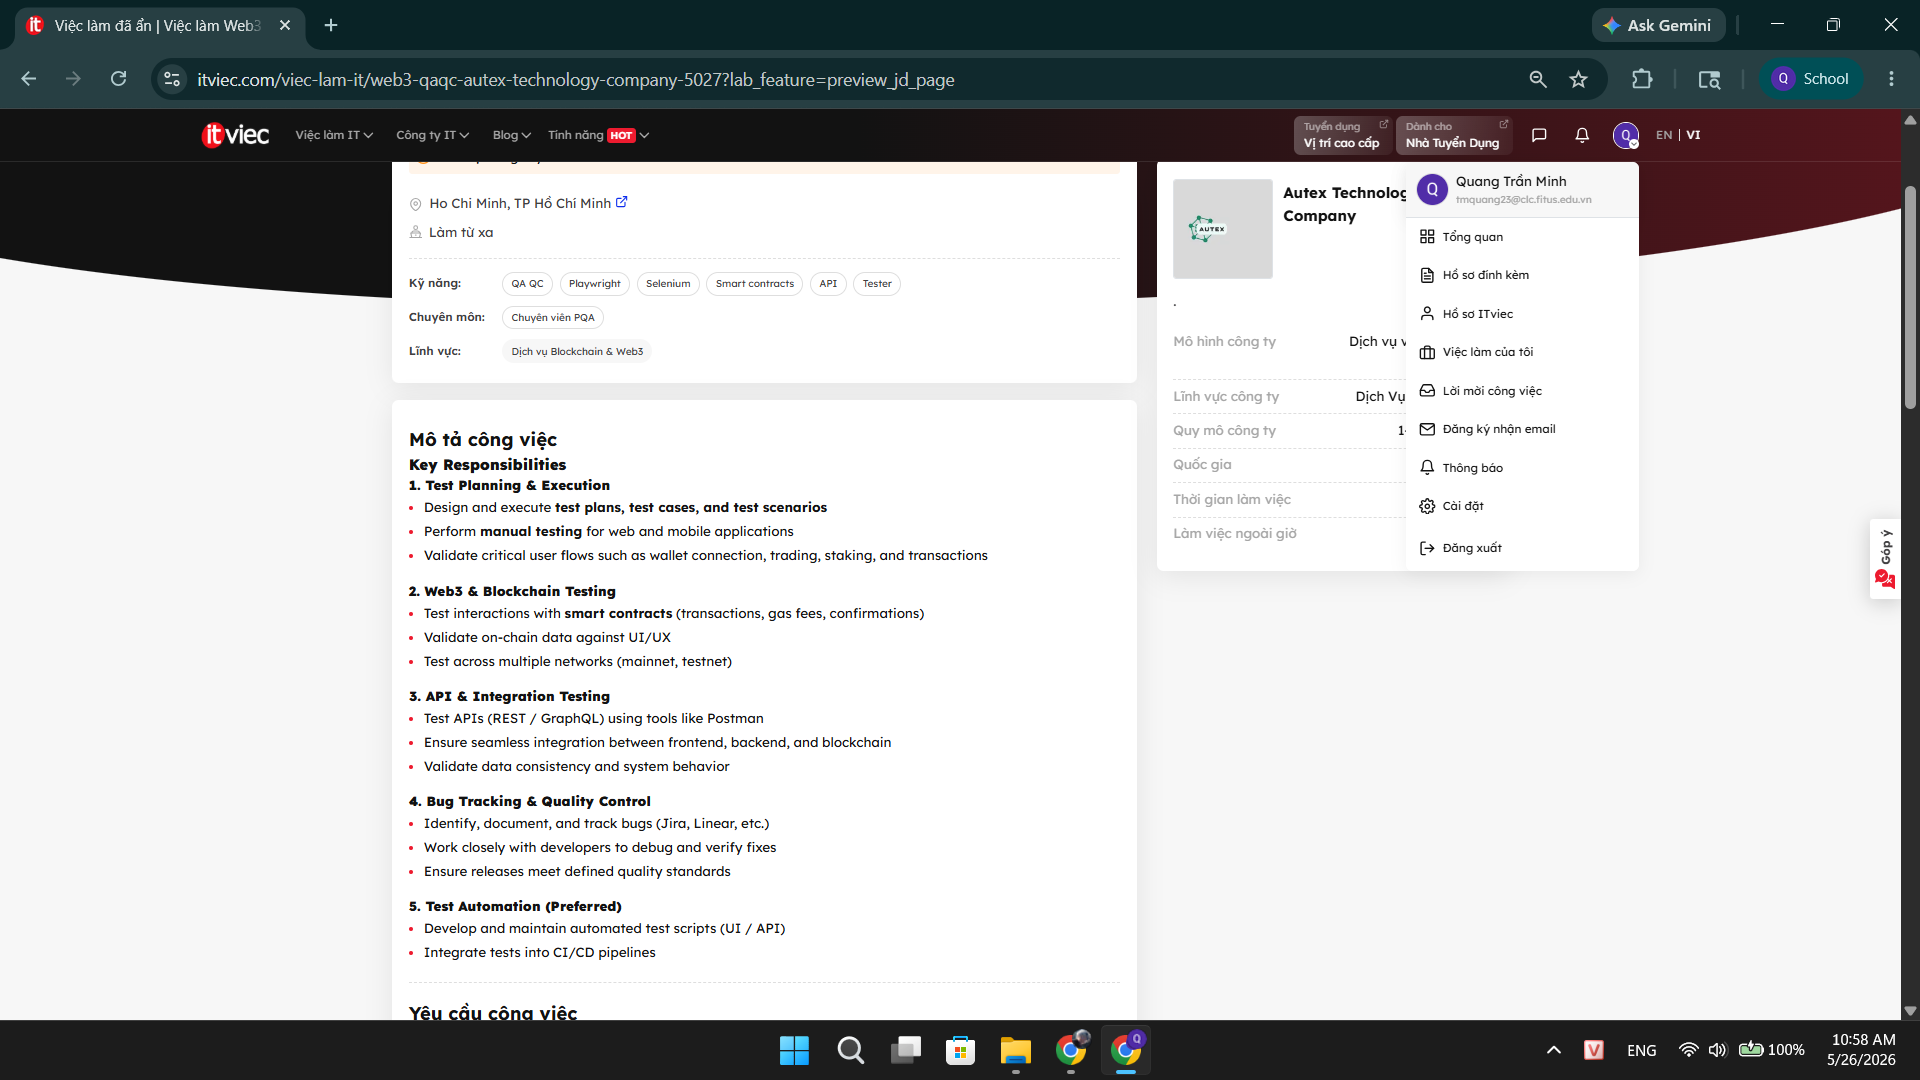
\includegraphics[scale=0.3]{pics_10_QA_QC_des/Web3_QAQC_des.png}
\end{center}

\subsubsection{Các kĩ năng yêu cầu}

\begin{center}
    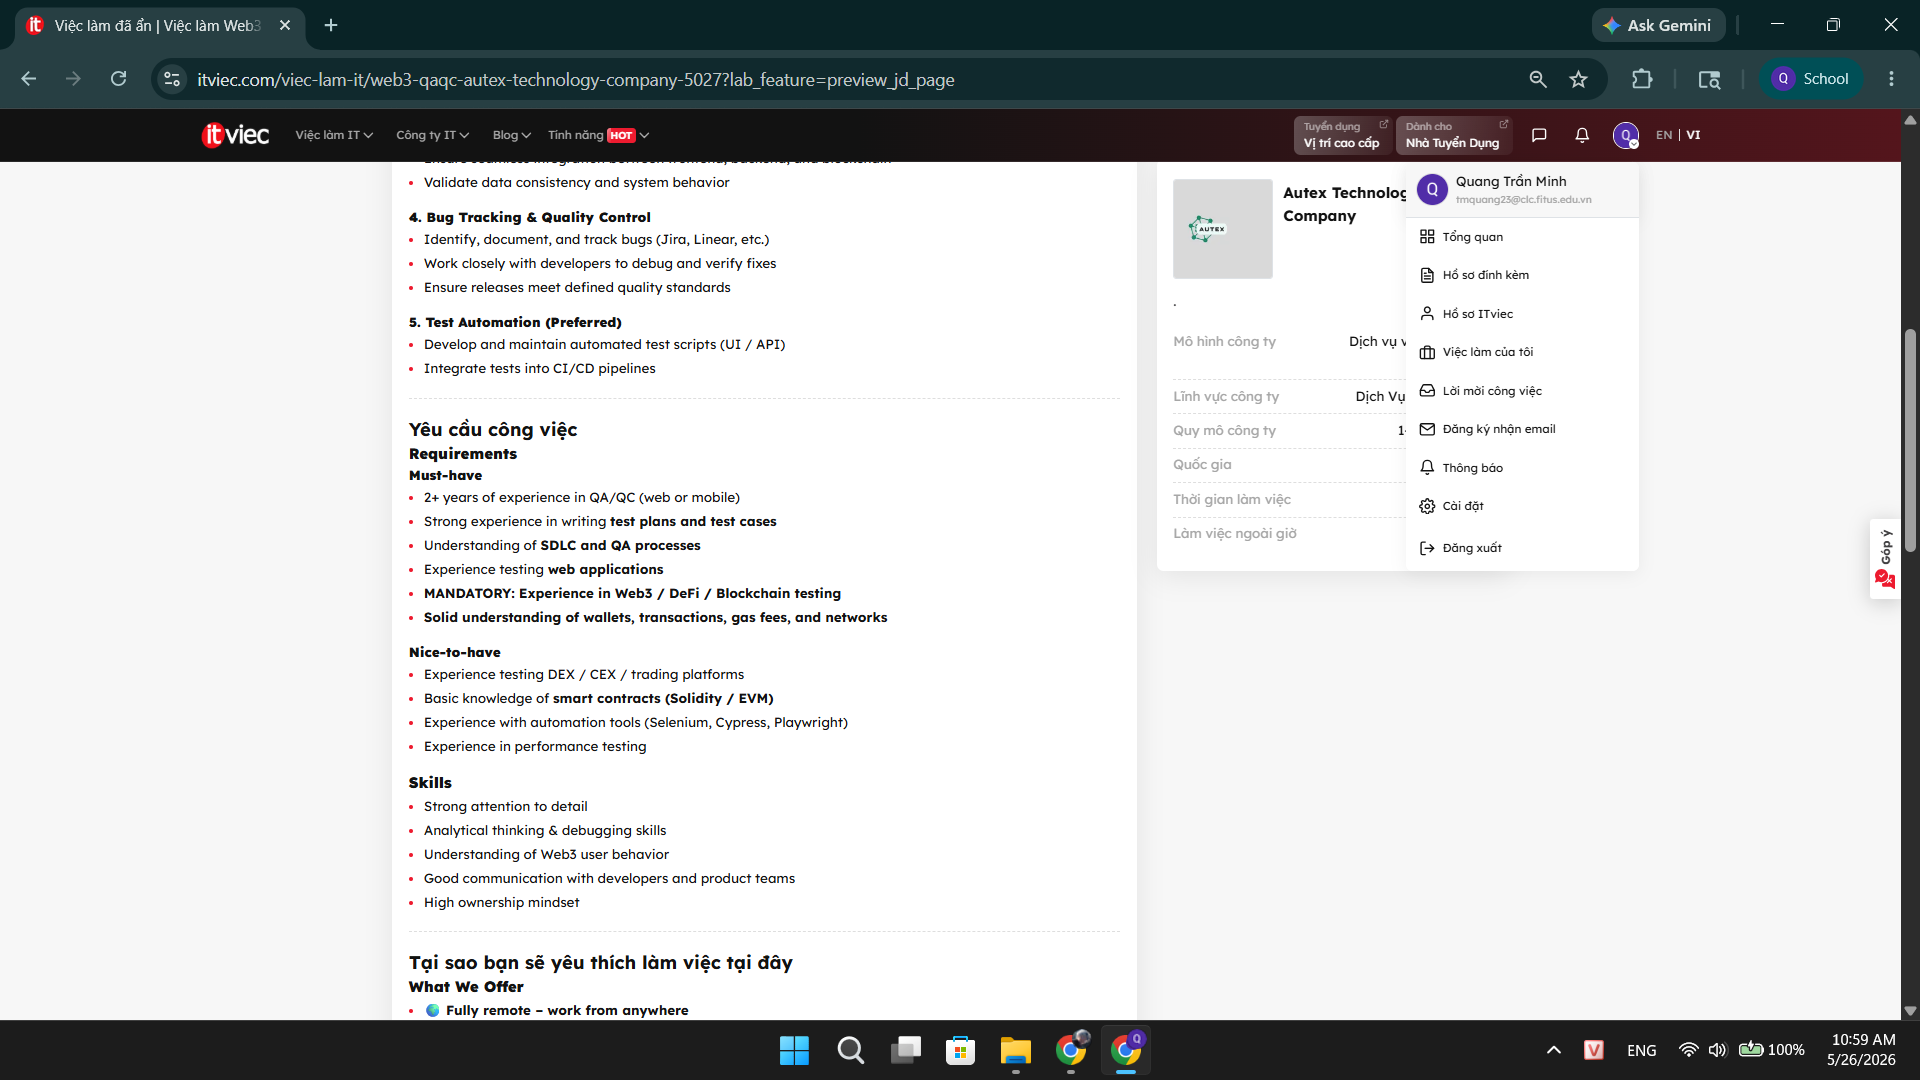
\includegraphics[scale=0.3]{pics_10_QA_QC_skilled/Web3_QAQC_skilled.png}
\end{center}

\subsubsection{Mức lương}

Salary in range: 1,500 - 2,500 USD

\subsubsection{Phân tích tác động của AI}

Công nghệ AI có tác động lên vai trò QAQC trong Web3 khi nó tự động hóa các công việc kiểm thử thường xuyên như xác minh dữ liệu trên chuỗi, kiểm tra gas fees và tương tác smart contract, tuy nhiên, khó khăn ở đây là AI vẫn chưa đủ thông minh để nhận biết ngữ cảnh phi tập trung và hành vi của người dùng Web3. Vì vậy, thay vì e ngại khả năng bị thay thế, QA Web3 nên tận dụng AI để tạo ra test case cho các kịch bản phức tạp và tập trung vào kiểm thử khám phá và bảo mật.